% Generated from paper/PAPER_DRAFT.md by scripts/build-integrated-paper.py
% Options for packages loaded elsewhere
\PassOptionsToPackage{unicode}{hyperref}
\PassOptionsToPackage{hyphens}{url}
\PassOptionsToPackage{dvipsnames,svgnames,x11names}{xcolor}
\documentclass[
  11pt,
]{article}
\usepackage{xcolor}
\usepackage[margin=1in]{geometry}
\usepackage{amsmath,amssymb}
\setcounter{secnumdepth}{5}
\usepackage{iftex}
\ifPDFTeX
  \usepackage[T1]{fontenc}
  \usepackage[utf8]{inputenc}
  \usepackage{textcomp} % provide euro and other symbols
\else % if luatex or xetex
  \usepackage{unicode-math} % this also loads fontspec
  \defaultfontfeatures{Scale=MatchLowercase}
  \defaultfontfeatures[\rmfamily]{Ligatures=TeX,Scale=1}
\fi
\usepackage{lmodern}
\ifPDFTeX\else
  % xetex/luatex font selection
\fi
% Use upquote if available, for straight quotes in verbatim environments
\IfFileExists{upquote.sty}{\usepackage{upquote}}{}
\IfFileExists{microtype.sty}{% use microtype if available
  \usepackage[]{microtype}
  \UseMicrotypeSet[protrusion]{basicmath} % disable protrusion for tt fonts
}{}
\makeatletter
\@ifundefined{KOMAClassName}{% if non-KOMA class
  \IfFileExists{parskip.sty}{%
    \usepackage{parskip}
  }{% else
    \setlength{\parindent}{0pt}
    \setlength{\parskip}{6pt plus 2pt minus 1pt}}
}{% if KOMA class
  \KOMAoptions{parskip=half}}
\makeatother
\usepackage{longtable,booktabs,array}
\newcounter{none} % for unnumbered tables
\usepackage{calc} % for calculating minipage widths
% Correct order of tables after \paragraph or \subparagraph
\usepackage{etoolbox}
\makeatletter
\patchcmd\longtable{\par}{\if@noskipsec\mbox{}\fi\par}{}{}
\makeatother
% Allow footnotes in longtable head/foot
\IfFileExists{footnotehyper.sty}{\usepackage{footnotehyper}}{\usepackage{footnote}}
\makesavenoteenv{longtable}
\usepackage{graphicx}
\makeatletter
\newsavebox\pandoc@box
\newcommand*\pandocbounded[1]{% scales image to fit in text height/width
  \sbox\pandoc@box{#1}%
  \Gscale@div\@tempa{\textheight}{\dimexpr\ht\pandoc@box+\dp\pandoc@box\relax}%
  \Gscale@div\@tempb{\linewidth}{\wd\pandoc@box}%
  \ifdim\@tempb\p@<\@tempa\p@\let\@tempa\@tempb\fi% select the smaller of both
  \ifdim\@tempa\p@<\p@\scalebox{\@tempa}{\usebox\pandoc@box}%
  \else\usebox{\pandoc@box}%
  \fi%
}
% Set default figure placement to htbp
\def\fps@figure{htbp}
\makeatother
\setlength{\emergencystretch}{3em} % prevent overfull lines
\providecommand{\tightlist}{%
  \setlength{\itemsep}{0pt}\setlength{\parskip}{0pt}}
\usepackage[]{natbib}
\bibliographystyle{unsrtnat}
\usepackage{bookmark}
\IfFileExists{xurl.sty}{\usepackage{xurl}}{} % add URL line breaks if available
\urlstyle{same}
\hypersetup{
  pdftitle={Learning Distributed Algorithms from Algorithmic Teachers},
  pdfauthor={Research collaboration (author order pending)},
  colorlinks=true,
  linkcolor={Maroon},
  filecolor={Maroon},
  citecolor={Blue},
  urlcolor={Blue},
  pdfcreator={LaTeX via pandoc}}

\title{Learning Distributed Algorithms from Algorithmic Teachers}
\author{Research collaboration (author order pending)}
\date{23 October 2026}

\setlength{\emergencystretch}{3em}
\setlength{\tabcolsep}{4pt}
\begin{document}
\maketitle

Unpublished integrated research draft, 23 October 2026. Author list and
order remain to be agreed. Historical contributions are attributed by
Git provenance.

\section*{Abstract}\label{abstract}
\addcontentsline{toc}{section}{Abstract}

Learning a distributed algorithm can mean predicting its actions,
reproducing its transitions, solving its task, matching its running
time, or generating the same probability law over solutions. These
objectives need not coincide. We investigate distributed graph coloring
through seven explicitly scoped algorithmic teachers and shared neural
policies. A historical five-seed architecture study finds that
normalized node/color networks, DeepSets palette scorers and local
palette Transformers each complete all 1,520 held-out evaluations, while
aggregation and representation controls expose failures. A complementary
seven-teacher study shows that almost-perfect local action accuracy can
coexist with substantial autonomous failure. We integrate the three
palette architectures with every native teacher, add small and
no-communication controls, and train 70 balanced short-budget replicas.
We separately audit teacher safety and termination, compare independent
scalar specifications on 103 small graph representatives, and
distinguish supplied arithmetic and schedules from learned decisions.
Statistical reconciliation aligns the compared output laws and shows
agreement between two procedures on six identical archival banks. Fresh
known-law controls reveal a large power difference for localized
alternatives. Our evidence supports a scoped separation between
functional generalization and fidelity to a teacher's complete solution
law. Missing historical collaborator weights prevent a complete
numerical replay of that cohort; no conclusion imputes those artifacts
or turns a nonrejection into equality.

A separate controlled-supervision study trains 735 fresh policies across
seven teachers, three architectures, seven label budgets and five
training seeds. Its strict benchmark certifies 12 of 21
teacher/architecture packages only when all five policies complete 1,000
final executions each without failure. Explicit information regimes,
nonmonotone per-seed curves and fixed-label optimization controls
separate this finite empirical certification from universal correctness
and theoretical sample-complexity claims.

A counterfactual extension adds admissible phase-specific oracles and
fixed-label optimization controls. It closes all nine previously pending
teacher/core packages on fresh five-policy, 1000-execution batteries
while preserving the twelve historical certifications. Concordant
controls also close those cells; counterfactual continuation fidelity
and required optimizer effort differ. Complete-output coupling,
information ablations and larger-graph transfer delimit what functional
success establishes.

\section{Introduction}\label{introduction}

A distributed coloring algorithm is an executable local rule embedded in
a communication model. A neural learner trained from its trajectories
must represent that rule, survive the states induced by its own
decisions, and remain meaningful when the number of neighbors or colors
changes. A proper coloring at the end of an execution is one useful
outcome, but it leaves several questions unanswered. Did the network
make the same decisions? Did it use the same information? Did it
preserve the teacher's progress guarantee? Did it sample the same
coloring distribution?

These questions become sharper when teachers differ. Random trials use
private randomness to resolve conflicts; priority rules exploit distinct
identifiers; color-wise preferences compare several possible colors;
auxiliary color reduction uses finite-field representations; speculative
programs repair temporary conflicts; and sequential greedy coloring
assumes a supplied order. A common neural interface can compare their
local decisions only if those differences remain explicit. Equal
parameter counts do not compensate for different supplied information or
computational schedules.

We study five notions of learning: \textbf{action fidelity}, agreement
on common teacher states and private inputs; \textbf{transition
fidelity}, agreement of updated states; \textbf{functional validity},
producing a proper complete coloring; \textbf{complexity fidelity},
preserving an appropriate teacher-specific cost; and
\textbf{distributional fidelity}, agreement of the probability laws of
complete solutions on a fixed labeled graph. The central question is how
these notions relate across teacher, architecture and evaluation regime.

The project combines two complementary lines. The degree-generalization
studies emphasize variable palettes, neighborhood aggregation,
conditional safety/progress and full labeled output distributions. The
native-teacher studies emphasize distinct algorithms, supplied phase
interfaces, local imitation and autonomous size transfer. Their results
are not pooled as if they used one protocol. Instead we reconstruct the
definitions, preserve their separate cohorts and add a balanced
integration experiment.

We add a second central axis: how much supervision each architecture
needs to achieve perfect functional performance within a defined
benchmark. An acquired node/action-component label is counted separately
from a trajectory, round, data replay or optimizer update. Information
compatibility precedes the comparison. The primary empirical gate
requires all five independently trained policies to complete every final
execution without a single failure; the observation and optimization
budgets remain separate experimental factors.

Our strongest conclusion is deliberately qualified: some learned local
policies generalize functionally while differing from their teacher in
observable full-output laws. This is not a claim that every successful
model must differ, or that every difference can be detected at our
sample sizes. Symmetry can force equality on particular graphs, and a
valid coupling can certify approximate agreement on a fixed graph. A
coherent account must accommodate all of these outcomes.

\subsection{Contributions and their
status}\label{contributions-and-their-status}

First, we specify a teacher/architecture interface preserving seven
native action alphabets and their supplied information. E1, DeepSets and
local palette attention are represented for each teacher, with a
controlled short-budget experiment and two additional baselines. This is
a framework and empirical study, not seven newly invented distributed
algorithms.

Second, we provide conditional proofs for the coded exact teacher rules,
an independent scalar transition audit and explicit limits of finite
testing. A repaired input-domain guard has a saved failing regression.
We separate correctness of a mathematical teacher from correctness of an
arbitrary trained numerical policy.

Third, we reconcile the statistical objects before comparing findings.
Matched-bank replays preserve original statistics; fresh known-law
controls quantify a finite-sample sensitivity difference. Existing
factorial data add observable-event bounds and size/degree interactions
without asserting a monotone law for total variation.

Fourth, the repository supplies an evidence ledger, complete scientific
audit, frozen checkpoint manifests, historical negative results,
executable reproduction commands and remotely verified recovery
artifacts. Historical collaborator checkpoint-level reproduction remains
explicitly incomplete.

\section{Related work}\label{related-work}

Neural algorithmic reasoning studies learned execution of algorithmic
computation \citep{velickovic2021nar}. CLRS supplies a common benchmark
spanning classical algorithm families \citep{velickovic2022clrs}. Our
question focuses on repeated local decisions in specified distributed
interpreters, including randomness and stopping semantics, and evaluates
a solution law as well as task success. We do not claim that trajectory
imitation or algorithmic generalization is new.

Distributed locality restricts the information available within a
bounded communication radius \citep{linial1992locality}. Connections
between local algorithms and GNN expressiveness clarify the importance
of inputs, depth and aggregation
\citep{sato2019approximation, loukas2020depth}. Those results do not
imply that a particular optimized network generalizes correctly. Our
controlled observations and conditional proofs concern explicit
architectures and teachers, rather than a universal GNN expressivity
theorem.

Deep Sets gives a principled shared-function/pooling construction for
sets \citep{zaheer2017sets}, while attention supplies content-dependent
interaction \citep{vaswani2017attention}. Here both act over each node's
palette; graph communication remains a neighborhood operation. Our
positional palette features retain color-name information, so these
models must not be described as fully color-permutation invariant.

Imitation learning encounters a state-distribution shift when learner
actions affect later observations \citep{ross2011dagger}. We use teacher
trajectories and counterfactual COMMIT labels, and evaluate autonomous
rollouts. This is not equivalent to on-policy dataset aggregation. Work
on asynchronous GNN inference also warns that synchronized behavior need
not survive changed execution semantics \citep{solodova2025hogwild};
this paper does not test asynchronous correctness.

The teachers draw on randomized coloring
\citep{luby1993randomness, johansson1999coloring}, priority coloring
\citep{jones1993parallel}, polynomial and iterative reduction
\citep{linial1992locality, kuhn2006complexity, barenboim2008linear},
color-wise preference trials \citep{schneider2010symmetry} and
speculative repair \citep{gebremedhin2000scalable}. We state the
implemented specialization rather than transferring the full complexity
guarantee of each cited paper.

Kernel two-sample tests compare probability laws through MMD
\citep{gretton2012kernel}. Characteristicness is an identifiability
property, not a finite-sample power guarantee. Random-permutation
calibration and familywise correction require their own assumptions
\citep{hemerik2018exact, holm1979simple}. Our honest witness omnibus is
a specified empirical instrument; no general minimax optimality or
universal dominance is claimed. This is a scoped primary-source review,
checked on 23 October 2026, rather than an exhaustive novelty
determination.

\section{Formal model and notions of
fidelity}\label{formal-model-and-notions-of-fidelity}

Let \(G=(V,E)\) be a fixed finite simple undirected labeled graph,
\(n=|V|\), and let \(C_v\) be the allowed colors of vertex \(v\). A
state contains a partial coloring \(q_v\in C_v\cup\{-1\}\) and any
explicitly declared auxiliary variables. A proper partial state has no
equal fixed colors across an edge. For permanent-color trial teachers,

\[ A_v(q)=C_v\smallsetminus\{q_u:u\in N(v),q_u\ge0\}. \]

In the local-palette studies, \(C_v=\{0,\ldots,d(v)\}\). Native
degree-three comparisons use a common \(C_v=\{0,1,2,3\}\) even at
vertices of lower degree. The two settings coincide on cubic graphs and
generally differ on irregular ones. No common maximum-degree input is
supplied to the local-palette E1 policy. Some native adapters explicitly
use the known bound 3.

A protocol step maps a current state and private input to participation
\(B\), candidate \(C\), confirmation \(J\), an auxiliary choice, or a
repair mark, according to its native phase. A permanent fixation is
applied only at a pending, permitted participating node with a candidate
and positive COMMIT. Palette range, pending-node gating, native phases
and schedules are supplied mechanisms; availability and conflict
decisions are learned unless explicitly identified as an exact-teacher
baseline.

For a frozen teacher \(T\) and policy \(M\), action fidelity evaluates
their decisions on identical input states and explicit random arrays.
Transition fidelity also evaluates the resulting states. Functional
success is the event that all vertices receive an allowed color and
every edge has different endpoint colors. These three predicates need
not coincide. A policy may produce another valid solution after its
first action disagreement; an inaccurate decision may instead propagate
to a later conflict.

For cutoff \(R\), write \(S_R\) for proper completion and
\(P_{T,R}^G=\mathcal L(X_G\mid S_R)\), where \(X_G=(c_1,\ldots,c_n)\).
Vertex and color names remain fixed. A joint terminal law instead
observes colors, partial outcomes and status at \(R\). A quotient law
canonicalizes color names. These are different estimands. If
\(P(S_R)=0\), the conditional solution law is undefined and cannot be
estimated by resampling until success.

Total variation is \(\operatorname{TV}(P,Q)=\sup_A|P(A)-Q(A)|\). A
statistically significant fixed-event difference therefore gives a TV
lower bound. For any valid coupling \((X,Y)\),
\(\operatorname{TV}(P,Q)\le P(X\ne Y)\) instead gives an upper bound.
Large disagreement under a poor coupling supplies no lower bound. In
particular, shared-randomness action fidelity and solution-law fidelity
are distinct questions.

\section{Algorithmic teachers}\label{algorithmic-teachers}

\textbf{Table 1. Implemented teachers and computational scope.} All
native comparisons below have degree\(\le\) 3 and global K4. Their exact
references and proof assumptions are expanded in AppendixA and the
teacher-audit document.

{\def\LTcaptype{none} % do not increment counter
\begin{longtable}[]{@{}
  >{\raggedright\arraybackslash}p{(\linewidth - 4\tabcolsep) * \real{0.3333}}
  >{\raggedright\arraybackslash}p{(\linewidth - 4\tabcolsep) * \real{0.3333}}
  >{\raggedright\arraybackslash}p{(\linewidth - 4\tabcolsep) * \real{0.3333}}@{}}
\toprule\noalign{}
\begin{minipage}[b]{\linewidth}\raggedright
Teacher
\end{minipage} & \begin{minipage}[b]{\linewidth}\raggedright
Local decision
\end{minipage} & \begin{minipage}[b]{\linewidth}\raggedright
Supplied information and cost convention
\end{minipage} \\
\midrule\noalign{}
\endhead
\bottomrule\noalign{}
\endlastfoot
LUBY & Bernoulli 1/2 participation; random available rank; reject equal
neighboring proposals & Two exchanges per trial; no IDs needed \\
JOHANSSON & Always-active random available rank; reject equal
neighboring proposals & Common K4; two exchanges per trial \\
JP & Pending strict ID maxima take first free color & Fixed distinct
IDs; synchronous native rounds, capped 128 \\
COLOR\_TRIALS & Strict discrete preference winner per color; keep lowest
winning color & Preferences 0--3, availability exchange; repeated
subroutine \\
BE\_BASE\_D3 & Linial field-point reductions then KW recoloring & Phase
clock, polynomial evaluation and receiver-relative equalities
supplied \\
SPECULATIVE\_GM & Concurrent block assignment, same-slot detection,
serial repair & Four balanced blocks and writable schedule supplied;
intermediate conflicts allowed \\
GREEDY & One permitted vertex takes first free color & Sequential
ID-order schedule supplied \\
\end{longtable}
}

The word LUBY denotes the explicit coin-participation random-trial rule.
It does not mean that this repository implements every derandomization
or PRAM component of Luby's work. JOHANSSON uses a larger common initial
palette at lower-degree vertices; the original analysis permits larger
initial lists, but the output law differs from the smallest local-list
initialization. Repeated COLOR\_TRIALS substitutes a fixed global degree
bound for its neighborhood bound and omits RankingTrials. BE\_BASE\_D3
is the degree-three base construction with two explicit Linial steps,
not the high-degree recursive algorithm. GM and greedy retain schedules
that would require a separate distributed implementation if no scheduler
were supplied.

The four parallel trial/priority interpreters stop at 128 native steps.
BE uses its auxiliary phases; GM and greedy run their supplied
schedules. The historical canonical E1 behavior experiment uses cutoff
256 and continues after a collision. We retain these differences rather
than calling all reported native steps a common LOCAL running time.

\section{Neural policies}\label{neural-policies}

\subsection{E1 NORMALIZED}\label{e1-normalized}

For each vertex/color pair define pending status \(u_v\) and ownership
\(o_{vc}=\mathbf1[q_v=c]\). Shared learned functions send a nonnegative
message and form a local state,

\[m^1_{vc}=\phi_1(u_v,o_{vc}),\qquad
h_{vc}=\psi_1(u_v,\max_{w\in N(v)}m^1_{wc}).\]

Availability is learned as \(\alpha_{vc}=\sigma(a(h_{vc}))\). The
ordered prefix \(S_{vc}=\sum_{j<c}\alpha_{vj}\) and
\(D_v=\max(\sum_j\alpha_{vj},.5)\) give normalized endpoints
\(L_{vc}=S_{vc}/D_v\), \(U_{vc}=(S_{vc}+\alpha_{vc})/D_v\). A shared
scorer reads \(h,\alpha,L,U,r_v^c\); the candidate is the maximum
scoring palette slot. Occupied colors are not removed by an exact mask.

The second exchange represents pending/ownership/participation/offer
bits. A learned COMMIT head reads the candidate slot after neighbor MAX.
Its prediction is applied without an exact safety veto. Canonical E1 has
16,035 parameters with hidden/message dimensions 64/32. This count is
independent of palette size, but messages, memory and computation grow
with the palette; each directed edge carries 32K floats per message
stage in the direct implementation.

\subsection{DeepSets and local palette
attention}\label{deepsets-and-local-palette-attention}

Both variants retain learned neighborhood messages, availability and
COMMIT. DeepSets replaces ordered-prefix scoring with shared per-slot
features and a mean of learned palette features. LocalPaletteTransformer
projects slots to dimension 16 and uses two-head self-attention with a
32-dimensional feedforward layer and zero dropout. Its attention is
within one vertex's palette, not between arbitrary graph vertices.

Their slot inputs include learned availability, normalized color
position, inverse palette size and private randomness. Prefix-free is
therefore not position-free. All three models are vertex-equivariant in
the ideal shared-rule, invariant-aggregation model, while ordered
prefixes and positions generally break color-name permutation symmetry.
Floating-point backend probes support finite implementations but do not
prove universal numerical equivariance.

\subsection{Native teacher adapters and
baselines}\label{native-teacher-adapters-and-baselines}

The common native interface preserves Pedro's two-hop rooted
representation and exact action alphabets. LUBY/Johansson/greedy use the
unextended core. JP, ColorTrials, BE and GM retain supplied native
context residuals. The E1 version adds 3,361 parameters in those cases;
analogous context is retained for the other palette architectures.
ColorTrials selects its final candidate after the second message.
BE-Linial predicts a valid field point and computes the polynomial value
through declared local arithmetic. The DeepSets and Transformer masks
use the actual field/palette size, including mixed field 7/13 examples.

Two new controls use the same supervision and native action interfaces.
The \textbf{small} model reduces hidden/message dimensions to 8/4 inside
the normalized family. The \textbf{no-communication} control erases
received neighbor states, relations and masks while retaining own state
and supplied native permissions. It is an information ablation with the
same large core, not a claim of parameter minimality. Exact teachers are
zero-trainable-parameter task baselines. The earlier direct-action
36,719-parameter GNN remains a historical comparator; it uses different
representation/loss choices.

No architecture is called minimal merely because it has fewer
parameters. We distinguish a mathematical information limitation,
sufficiency within a tested architecture family, and finite empirical
success.

\section{Training and experimental
design}\label{training-and-experimental-design}

\subsection{Three distinct training
cohorts}\label{three-distinct-training-cohorts}

The historical mechanism study trains five seeds 41000--41004 per
primary architecture on 800 cubic N40 graphs, three teacher
trajectories,120 epochs, Adam at .001 and batch 128 round examples. The
full-graph E1 loss combines participation BCE, candidate cross-entropy,
and equal half-weights for own and counterfactual COMMIT supervision.
During ten warmup epochs COMMIT uses teacher proposals. Afterwards exact
labels are recomputed for the proposals actually queried; hard proposals
separate gradients into decision modules. Training states remain
teacher-generated. Rollout evaluation supplies the autonomous-state
test.

Pedro's native comparisons instead use five seeds 0--4, common immutable
pools of 800 cubic N40 graphs with three trajectories,17,760 updates and
batches of 1,680 eligible root decisions. The direct GNN uses
native-action losses. Its E1 follow-up uses 1,480 warmup updates and
native own/counterfactual confirmation labels. Star-local and full-graph
intervention samplers are different. The native follow-up also changes
BE's auxiliary representation. Consequently its architecture comparison
measures a training/representation package, not an isolated
architectural intervention.

The integrated extension uses 24 new cubic N40 graphs, one trajectory
each, eight validation graphs and two new seeds 73000--73001. Every
teacher has the same five architecture cells. Timing pilots selected 500
common updates of 128 root decisions, with 50 warmup updates, before
scientific pools were generated. This exposes 64,000 sampled root
decisions per model. It is intentionally a short-budget study, not a
repeat of 29,836,800-decision native training. All 70 final checkpoints
are retained without validation promotion or a second training budget
after observing outcomes. Compatible shared message/COMMIT initial
weights are preserved across the three large palette models within a
seed; the small family has different dimensions.

The two initialization replicas share teacher-specific data pools. They
do not replicate data generation, and repeated rollout tapes do not
create additional independently trained models. Hyperparameters,
parameter counts, source hashes, training time, data manifests and
checkpoint digests are recorded in
\texttt{results/integration/multiteacher/}.

\subsection{Evaluation and units of
replication}\label{evaluation-and-units-of-replication}

The full-budget architecture cohort contains 304 common graph/tape cases
per model, giving 1,520 cases for five seeds of one architecture. It
covers degree and size transfer, irregular/heterogeneous families,
cliques and structured controls. The native cohort contains 396 cases
per model through N10,240. Its E1 follow-up uses already-published cases
and is exploratory. Five seed outcomes on one graph are not five
independent graph instances.

The new native extension uses five independent graph specifications:
regular N16, irregular N40, regular N160, path 16 and K4, excluding
training/validation labeled fingerprints. Every exact teacher and
checkpoint produces 128 new independent executions on each graph. Full
color vectors, statuses, native steps, failure labels and random seeds
are archived. The graph ensemble is small and fixed; no confidence
interval treats it as a representative sample of all graphs.

Participation, candidate and COMMIT accuracy use common teacher states
and explicit private inputs. Native COMMIT labels retain their own
semantics: ColorTrials preference rejection is not identical to a
physical collision; GM assignment can deliberately create simultaneous
conflicts before repair. Per-phase action accuracy, component
denominators and GM mark counts are retained so WAIT or negative-mark
imbalance cannot alone establish learning.

Functional evaluation applies the model's own decisions, with native
permissions but no oracle conflict veto. We report invalid outputs and
incomplete outcomes alongside successes. Mean native steps over all
attempts can be reduced by early failure; efficiency comparisons
therefore also use successful outputs and remain within one teacher.
Parameter count, training CPU time and native steps measure different
costs. No deployment latency or cross-teacher LOCAL speed ranking is
inferred.

\subsection{Distributional inference}\label{distributional-inference}

The primary observation is an independent complete run. For the
historical local-list studies, V2 splits the valid completed prefix into
selection and evaluation subsets, fits bounded witnesses on selection
only, and calibrates their joint maximum with a full-vector MMD
component on evaluation rows. Every permutation acts jointly on complete
row labels; vertex columns are never independently shuffled. Pooled
scaling ignores evaluation source labels. The permutation count 19,999
gives minimum p .00005.

The factorial primary family has 720 graph/checkpoint hypotheses and the
robust study 795. Event, irregular-graph, historical-replication and
explanation families remain separate. For the new extension, all 350
planned teacher/model/ graph comparisons form one Holm family. Every
model is compared with its own teacher's exact reference. A cell with
fewer than four valid completed rows is untestable and assigned p 1 only
for planned-family bookkeeping. It is not an equality result.
Conditioning, failure frequencies and the native cause of termination
remain visible.

Pedro's separate behavior experiment uses a mixture of Hamming kernels
and terminal-status equality, plus family/size-stratified permutation
aggregation. It also tests a color-name quotient and obtains
coupling-based TV upper bounds. We audit its exact statistic and compare
procedures on matched rows, without pooling its hypothesis family with
our graph-specific families.

\section{Conditional correctness and representation
results}\label{conditional-correctness-and-representation-results}

\textbf{Proposition 1 (safety and progress are separate).} For a proper
partial state, candidates supported on available colors and exact
rejection of simultaneous equal neighboring offers preserve properness.
This alone does not imply a uniform progress or termination bound.

\emph{Proof.} A new color avoids old fixed neighbors by availability,
and two adjacent equal proposals cannot both be confirmed. This proves
safety by induction. In an all-free K-clique, suppose every node
proposes color 0 and participates independently with probability 1/2. A
node confirms only when it is the unique participant, so the probability
that any node advances is \(K/2^K\). Waiting for the first confirmation
has mean \(2^K/K\). A policy that always waits never terminates. Safety
thus supplies no constant progress bound. The example concerns specified
policies, not every learned checkpoint. \(\square\)

\textbf{Proposition 2 (exact teacher guarantees on the declared
domain).} Under fresh independent ideal private randomness and the
hypotheses in Table 1, the uncapped LUBY, JOHANSSON and repeated
ColorTrials teachers preserve properness and terminate almost surely,
with O(log n) expected native rounds at degree\(\le\) 3. JP is safe and
terminates within n uncapped native rounds. BE\_BASE\_D3
deterministically reaches four auxiliary colors in 15 native steps.
Greedy and synchronized speculative GM terminate under their supplied
schedules and produce proper final colorings.

\emph{Proof sketch; complete arguments in AppendixA.} Availability
satisfies \(|A_v|\ge d_U(v)+1\). LUBY has conditional progress at least
1/4 using the independent candidate product and Jensen's inequality. For
JOHANSSON each pending neighbor has at least two available colors,
giving the sufficient degree-three bound 1/8. For ColorTrials, the event
that a vertex has preference 3 for a free color and all at most three
competitors have preference\(\le\) 2 has probability at least 27/256. A
uniform positive conditional progress bound\(\rho\) gives
\(P(T>t)\le n(1-\rho)^t\) by iterated conditioning and union bound. JP's
eligible maxima form an independent set and include a maximum pending
ID. Polynomial reductions preserve proper auxiliary colors; KW uses
disjoint four-color blocks. Sequential first fit and the last-repaired
endpoint argument complete the remaining cases. Finite caps are distinct
from these uncapped guarantees. \(\square\)

\textbf{Proposition 3 (a finite-type sufficient COMMIT certificate).}
For the canonical MAX architecture, assume nonnegative deterministic
shared messages, zero empty aggregation, legal candidate-slot gathering
and pending/participation gating. A participating pending center's
neighbor slot has six possible legal types. If the COMMIT logit has the
correct strict sign on all 64 subsets of these types, it implements
exact rejection at arbitrary degree and palette in real arithmetic.

\emph{Proof.} Componentwise MAX is commutative, associative and
idempotent, so only the set of present types matters, not
multiplicities. The gather retains only the own candidate slot. Fixed
ownership of that color and simultaneously participating equal offers
are the two forbidden types. The 64-set sign table is therefore
sufficient. It does not establish candidate diversity or termination.
Native continuous-ID/context extensions are not automatically covered by
this alphabet. Interval computations and floating-point error
assumptions are documented separately. \(\square\)

\textbf{Proposition 4 (a scoped information limitation).} A
deterministic policy given only its own color/pending status and private
draw cannot reproduce all arbitrary-state first-free decisions without
neighbor information. Further, in the memoryless current-state
interface, some random-trial COMMIT decisions require information beyond
radius one.

\emph{Proof.} A pending center with the same own inputs but a fixed
neighbor of color 0 versus 1 has different first-free colors; its
identical local input cannot prescribe both. For the radius example use
path 0--1--2, with 0 and 1 pending and 2 fixed at 1 in one state and 2
in the other. Let both pending vertices participate, with candidate
draws .3 at 0 and .4 at 1 in common K4. Vertex 0 proposes 1 in both
states. Vertex 1 proposes 2 in the first state and 1 in the second,
changing vertex 0's COMMIT. Its radius-one initial states/private inputs
agree. This lower bound assumes no previously stored neighbor
availability or supplied free-color flags. It is not a lower bound for
every coloring algorithm, every persistent-memory protocol or every
scheduling model. \(\square\)

\textbf{Proposition 5 (clique conditional-law equality).} On K\_n with
exactly n colors, any vertex-equivariant protocol with exchangeable
private input and positive probability of proper completion has the
uniform conditional law on the n! proper labeled color vectors.

\emph{Proof.} Equivariance and exchangeability give a vertex-invariant
trajectory law by induction. The proper-completion event is invariant,
so conditioning preserves this invariance. Vertex permutations act
transitively on all proper n-color vectors. All conditional masses are
therefore equal. Different candidate rules can satisfy the same
conclusion. This is not proved by finite nonrejection and need not hold
on other graphs. \(\square\)

\textbf{Proposition 6 (observable and coupling bounds).} A simultaneous
interval \([l,u]\) for \(P_M(A)-P_T(A)\) gives
\(\operatorname{TV}(P_M,P_T)\ge\max(0,l,-u)\). A valid coupling gives
the upper bound \(\operatorname{TV}(P_M,P_T)\le P(X_M\ne X_T)\).

\emph{Proof.} The first inequality follows by restricting the supremum
defining TV to the eventA and propagating its confidence statement. For
the second, the difference of probabilities of any event is bounded by
the chance that the coupled outcomes disagree. Taking the supremum
proves the bound. Neither compares TV distances across
different-dimensional graph spaces. \(\square\)

\section{Learning across teachers: historical
evidence}\label{learning-across-teachers-historical-evidence}

\textbf{Table 2. Pedro's published full-budget native comparison.} Each
entry is successful graph/tape/checkpoint evaluations out of 1,980.
These aggregate counts are preserved historical evidence; their original
weights and raw output banks are missing here. The follow-up reuses
known test cases.

{\def\LTcaptype{none} % do not increment counter
\begin{longtable}[]{@{}lrr@{}}
\toprule\noalign{}
Teacher & Direct-action GNN & E1 / declared native adaptation \\
\midrule\noalign{}
\endhead
\bottomrule\noalign{}
\endlastfoot
LUBY & 1,857 & 1,980 \\
JOHANSSON & 1,919 & 1,980 \\
JP & 1,635 & 1,631 \\
COLOR\_TRIALS & 1,980 & 1,980 \\
BE\_BASE\_D3 & 872 & 1,980 \\
SPECULATIVE\_GM & 1,975 & 1,951 \\
GREEDY & 1,842 & 1,980 \\
\end{longtable}
}

These results establish no universal teacher ranking. E1/adaptations
improve the reported LUBY, Johansson, BE and greedy outcomes, leave
ColorTrials at complete observed success, and do not improve JP or GM.
BE's large change also changes auxiliary representation and training.
Both positive and negative before/after comparisons matter.

The JP E1 follow-up has mean local action accuracy .999735 but succeeds
in 1,631/1,980 autonomous evaluations. This directly illustrates
accumulation and state-distribution effects; it does not identify a
unique causal mechanism for every failure. The reported GM losses
similarly warn that exact local validation on sampled teacher states
need not guarantee all rare conflict marks in large autonomous
executions.

\section{Functional generalization and
aggregation}\label{functional-generalization-and-aggregation}

\textbf{Table 3. Full-budget historical architecture controls.} Five
independent training seeds share 1,520 held-out graph/tape/checkpoint
evaluations per architecture; the fixed evaluation instances are blocked
rather than treated as independent new graphs per seed.

{\def\LTcaptype{none} % do not increment counter
\begin{longtable}[]{@{}ll@{}}
\toprule\noalign{}
Architecture / intervention & Reported principal outcome \\
\midrule\noalign{}
\endhead
\bottomrule\noalign{}
\endlastfoot
E1 NORMALIZED & 1,520/1,520 proper completions \\
DeepSets palette & 1,520/1,520 proper completions \\
LocalPaletteTransformer & 1,520/1,520 proper completions \\
Raw endpoint control & Lost progress in 346 evaluations \\
SUM aggregation & Stalled in 1,196 evaluations \\
MEAN aggregation & Produced 839 improper final colorings \\
\end{longtable}
}

The normalized/raw-endpoint intervention preserves scorer tensor shapes,
initialization, data and update counts within seed, making it more
controlled than the earlier raw-prefix architecture comparison. SUM and
MEAN alter neighbor reductions and multiplicity handling. Their failures
are evidence about those implementations and training conditions, not a
proof that SUM or MEAN cannot represent any correct coloring policy.

The successful prefix-free models show that E1's original ordered
prefixes are not necessary for observed functional generalization in
this experiment. They still receive useful palette position information
and learned graph messages. No conclusion says that generic attention
alone supplies a distributed coloring algorithm. Constant parameter
count also does not imply constant communication or inference cost.

\section{Balanced teacher/architecture
extension}\label{balanced-teacherarchitecture-extension}

\textbf{Table 4. New balanced finite-cohort functional outcomes.} Each
model architecture/teacher cell pools two fixed initialization replicas,
five fixed graphs and 128 independent runs per graph/checkpoint,
totaling 1,280 attempts. The entries are counts of proper completions,
not population confidence bounds or full-budget architecture rankings.

{\def\LTcaptype{none} % do not increment counter
\begin{longtable}[]{@{}llllll@{}}
\toprule\noalign{}
Teacher & E1 & DeepSets & Transformer & Small & No messages \\
\midrule\noalign{}
\endhead
\bottomrule\noalign{}
\endlastfoot
Luby & 1,280 & 1,280 & 1,280 & 1,280 & 30 \\
Johansson & 1,280 & 1,280 & 1,280 & 0 & 0 \\
JP & 473 & 395 & 448 & 1 & 0 \\
ColorTrials & 1,280 & 1,280 & 1,280 & 640 & 0 \\
BE (base d 3) & 232 & 268 & 255 & 1 & 8 \\
Speculative GM & 1,156 & 1,170 & 1,155 & 444 & 0 \\
Greedy & 1,280 & 1,280 & 1,280 & 1,280 & 0 \\
\end{longtable}
}

Figure 1 displays the same finite-cohort percentages. Individual
seed/graph records, failure types and native steps are available in
\texttt{functional.csv} and the original hashed banks. The exact
reference uses one 128-run bank per teacher/graph shared across its
model comparisons; it is not counted twice to create extra reference
data.

\begin{figure}
\centering
\pandocbounded{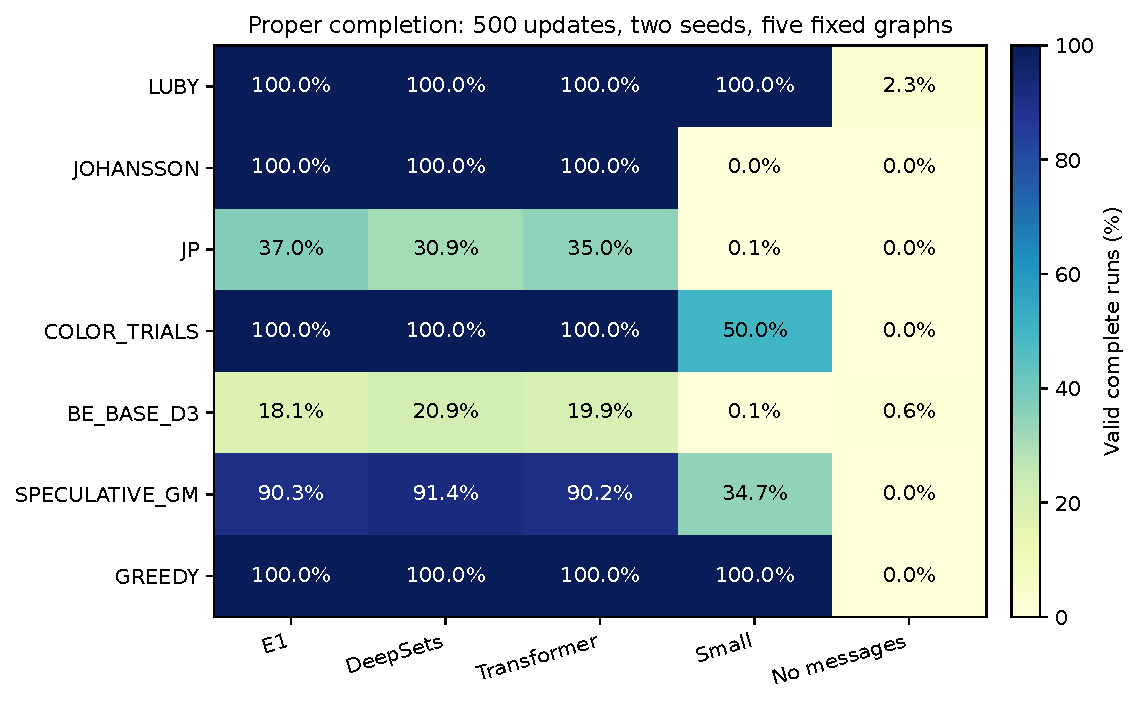
\includegraphics[keepaspectratio,alt={Proper-completion percentages on the balanced short-budget cohort. Every architecture receives 500 updates; each cell retains all failures and both training seeds.}]{figures/integration-functional.pdf}}
\caption{Proper-completion percentages on the balanced short-budget
cohort. Every architecture receives 500 updates; each cell retains all
failures and both training seeds.}
\end{figure}

All three large palette architectures completed 1,280/1,280 attempts for
each of LUBY, JOHANSSON, COLOR\_TRIALS, GREEDY. At the same short
budget, JP and BE retained substantial failures, while speculative GM
was intermediate. These differences compare specified
training/representation packages, not intrinsic teacher complexity.
Per-teacher architecture differences and both replicas remain in the
table; there is no universal winner.

The short budget and small training graph sample limit interpretation. A
failed cell can reflect optimization or coverage, and does not prove a
representational impossibility. A successful small model establishes
finite sufficiency within its family; it does not prove parameter
minimality. The no-communication control retains native permissions, so
its successes cannot be generalized to a scheduler-free anonymous
setting.

Figure 2 compares common-state local validation accuracy and autonomous
functional validity for all 70 separately trained models. Local
validation contains different phase/class mixtures across teachers, so
between-teacher horizontal comparisons require the per-phase
denominators. Each plotted point remains one checkpoint; rollout repeats
are not training replicas.

\begin{figure}
\centering
\pandocbounded{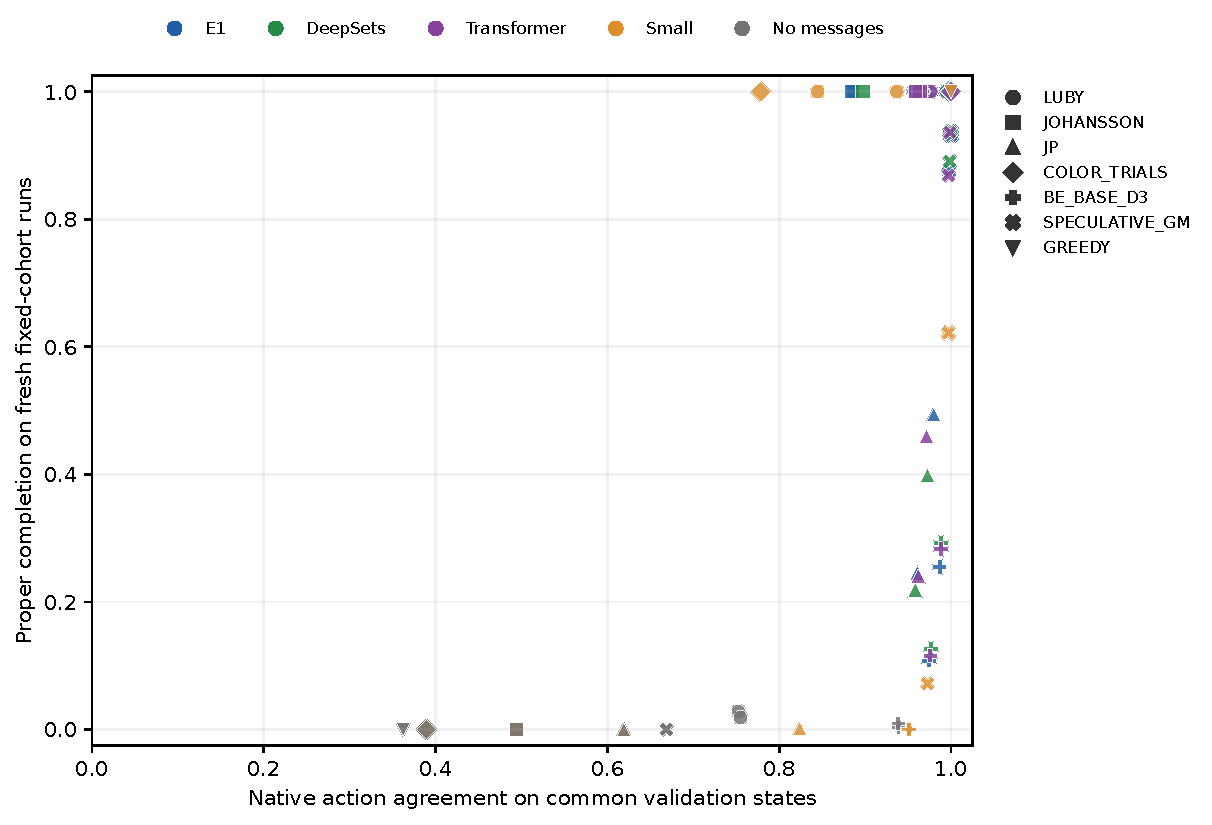
\includegraphics[keepaspectratio,alt={Common-state native action accuracy and autonomous proper-completion rate. Colors denote architectures and symbols teachers; all 70 checkpoints are plotted and identical points can overlap.}]{figures/integration-fidelity.pdf}}
\caption{Common-state native action accuracy and autonomous
proper-completion rate. Colors denote architectures and symbols
teachers; all 70 checkpoints are plotted and identical points can
overlap.}
\end{figure}

\section{Complete-coloring laws and statistical
reconciliation}\label{complete-coloring-laws-and-statistical-reconciliation}

\subsection{Historical local-palette
evidence}\label{historical-local-palette-evidence}

\textbf{Table 5. Separate historical global-law cohorts.} Counts are
rejections after each declared Holm family. They are decisions under
different cohorts, sample sizes and methods, not comparable numerical
distances.

{\def\LTcaptype{none} % do not increment counter
\begin{longtable}[]{@{}
  >{\raggedright\arraybackslash}p{(\linewidth - 6\tabcolsep) * \real{0.2000}}
  >{\raggedleft\arraybackslash}p{(\linewidth - 6\tabcolsep) * \real{0.2667}}
  >{\raggedleft\arraybackslash}p{(\linewidth - 6\tabcolsep) * \real{0.2667}}
  >{\raggedleft\arraybackslash}p{(\linewidth - 6\tabcolsep) * \real{0.2667}}@{}}
\toprule\noalign{}
\begin{minipage}[b]{\linewidth}\raggedright
Architecture
\end{minipage} & \begin{minipage}[b]{\linewidth}\raggedleft
Initial MMD:250 runs,265 comparisons
\end{minipage} & \begin{minipage}[b]{\linewidth}\raggedleft
Robust V2:500 attempts,265 comparisons
\end{minipage} & \begin{minipage}[b]{\linewidth}\raggedleft
Factorial V2:500 attempts,240 comparisons
\end{minipage} \\
\midrule\noalign{}
\endhead
\bottomrule\noalign{}
\endlastfoot
E1 NORMALIZED & 10 & 52 & 115 \\
DeepSets & 46 & 107 & 170 \\
Local palette Transformer & 127 & 181 & 180 \\
\end{longtable}
}

On identical new robust banks, the earlier single-scale MMD gives
21,71,147 rejections respectively; on identical factorial banks it gives
49,121,174. These matched-data comparisons isolate the procedure/budget
difference from historical new-bank variation. They still do not turn
rejection counts into a ranking of TV distances or make V2 uniformly
more powerful. Archived auxiliary cases include losses as well as gains
for V2.

The distributional differences coexist with strong functional
generalization in the full-budget architecture cohort. Functional
success restricts outputs to proper colorings but does not select a
unique probability law on that set. The teacher itself need not sample
proper colorings uniformly. Conversely, the clique symmetry argument
gives genuine scoped equality despite different proposal mechanisms.
Thus neither candidate mismatch nor success alone determines a
global-law conclusion.

\subsection{Reconciliation with the independent E1 behavior
study}\label{reconciliation-with-the-independent-e1-behavior-study}

Pedro reports no rejections among 100 primary
stratum/model/representation tests using five newly trained E1s,
degree\(\le\) 3, common K4, cutoff 256 and 256 runs per graph. His
experiment tests full labeled terminal vectors/status and a color-name
quotient. It is not the same checkpoint cohort, degree/palette regime,
cutoff or hypothesis family as Table 5. Ten labeled-law and eleven
quotient-law pairs obtain simultaneous TV\(\le\) .05 certificates using
coupling disagreement upper bounds. Those certificates are affirmative
fixed-graph approximate-equivalence statements; zero rejections alone
would not supply them. Their underlying raw banks and trained weights
are not available here.

We independently verify the mixture statistic's equality to unbiased MMD
and its inclusive permutation calculation. On identical archival 500-row
banks from the first regular N128/degree 3 graph, neither mixture MMD
nor V2 rejects any of the three s 41000 architecture comparisons. On the
first regular N512/degree 100 graph, both reject all three. Each
high-degree raw p-value is .00005; the exploratory six-test Holm value
is .0003, whereas the original 720-test V2 adjusted value remains .036.
The original statistics and p-values replay exactly. These are matched
historical reanalyses, not new independent confirmation or a replay of
Pedro's missing weights.

Different finite-sample power remains scientifically important. On a
star with 200 iid binary leaves, change only the center from uniform on
199 high colors to uniform on a 100-color subset. Every vector is a
proper local-list coloring, TV equals 99/199, and the mixture population
MMD\(^2\) is 9.569688e-6. Twenty fresh independent experiments per cell
give Table 6.

\textbf{Table 6. Independent matched-data controls, nominal alpha
.05,999 permutations.} Entries are detections out of 20 independent
experiments.

{\def\LTcaptype{none} % do not increment counter
\begin{longtable}[]{@{}lrrr@{}}
\toprule\noalign{}
Law & Runs per generator & Mixture MMD & Honest V2 \\
\midrule\noalign{}
\endhead
\bottomrule\noalign{}
\endlastfoot
Same-law star & 256 & 0 & 1 \\
Same-law star & 500 & 1 & 1 \\
Center-only alternative & 256 & 0 & 20 \\
Center-only alternative & 500 & 3 & 20 \\
\end{longtable}
}

For the alternative the pointwise exact 95\% power intervals
are{[}0,.1684{]} and{[}.0321,.3789{]} for the mixture and{[}.8316,1{]}
for V2 at both sizes. Figure 3 preserves the null controls and
uncertainty. This finite-law result does not establish strict
Holm-adjusted power for 720 hypotheses or explain every historical model
comparison. In particular, it does not show that Pedro's degree-three
neural laws exhibit this star alternative.

\begin{figure}
\centering
\pandocbounded{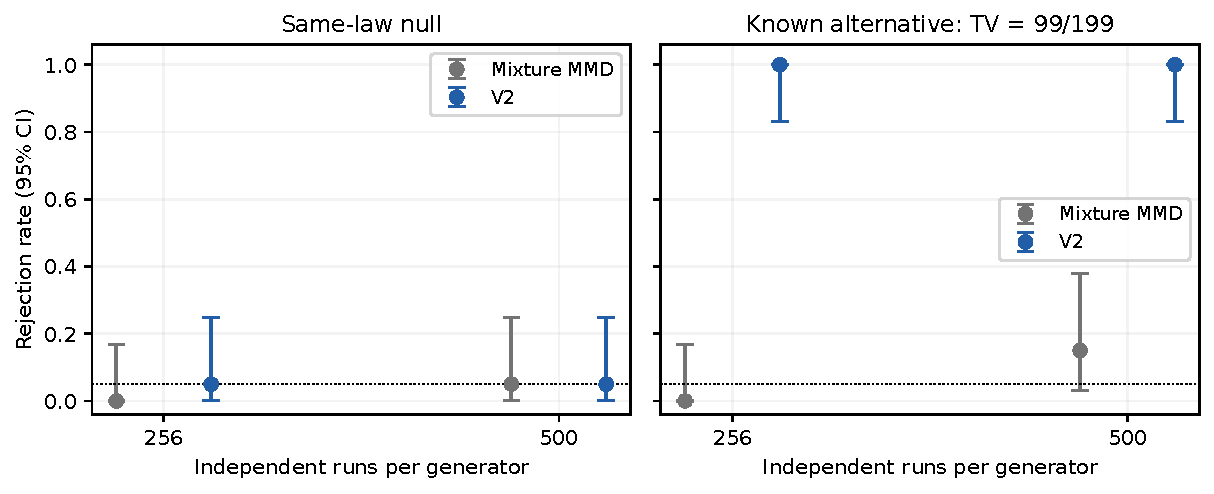
\includegraphics[keepaspectratio,alt={Independent known-law null and power checks. Both procedures receive identical fresh full-coloring rows in each trial; intervals are pointwise exact 95\% binomial intervals over 20 experiments.}]{figures/integration-power.pdf}}
\caption{Independent known-law null and power checks. Both procedures
receive identical fresh full-coloring rows in each trial; intervals are
pointwise exact 95\% binomial intervals over 20 experiments.}
\end{figure}

The discrepancy classification is consequently mixed: different output
representations are different definitions;
graph/palette/checkpoint/cutoff changes are protocol differences; the
known-law power gap is statistical; and the effect of V2 on Pedro's
exact original banks remains unresolved. No speculative explanation
closes that final gap. The complete audit is
\texttt{docs/integration/GLOBAL\_DISTRIBUTION\_RECONCILIATION.md}.

\subsection{New teacher-specific global
comparisons}\label{new-teacher-specific-global-comparisons}

Of 350 planned teacher/checkpoint/graph hypotheses, 227 are testable and
123 have fewer than four successful model/reference rows. After Holm
over the complete planned family, 6 reject. Each reference bank belongs
to the corresponding teacher. These counts concern conditional output
laws on a small fixed cohort; functional failures and limited power
remain separate.

All six new rejections concern two small checkpoints that nevertheless
complete all 640 of their functional evaluations: LUBY seed 73001 and
ColorTrials seed 73000. Each differs from its own teacher on three fixed
graphs, with raw p .00005 and Holm-adjusted p .0175. The LUBY core has
551 parameters and the context-extended ColorTrials model 1,560. This
supplies new finite-cohort evidence for functional/distributional
separation under two teachers. The other small ColorTrials
initialization fails all 640 functional attempts, so the successful
checkpoint is not presented as universal small-model robustness. The
large architectures have no new rejections here; those nonrejections do
not certify their law equality.

The native comparisons use the audited V2 selection/permutation
construction with an explicit global-K4 histogram alphabet. The
historical feature allocator assumed max(degree)+1 bins, which is
insufficient for valid four-color native path outputs. The first call
failed before producing a p-value. A separate adapter repairs that
allocation while preserving actual degrees, feature definitions and the
original frozen module. An independent color 3 path-null test and a
matching-alphabet exact replay verify the compatibility change. This is
documented as an integration repair, not an invalidation of the
historical local-list study. The new native power is not inherited from
its old validation by assertion.

\textbf{Table 7. New Holm rejections / testable comparisons (ten planned
per teacher and architecture).}

{\def\LTcaptype{none} % do not increment counter
\begin{longtable}[]{@{}llllll@{}}
\toprule\noalign{}
Teacher & E1 & DeepSets & Transformer & Small & No messages \\
\midrule\noalign{}
\endhead
\bottomrule\noalign{}
\endlastfoot
Luby & 0/10 & 0/10 & 0/10 & 3/10 & 0/2 \\
Johansson & 0/10 & 0/10 & 0/10 & 0/0 & 0/0 \\
JP & 0/8 & 0/7 & 0/7 & 0/0 & 0/0 \\
ColorTrials & 0/10 & 0/10 & 0/10 & 3/5 & 0/0 \\
BE (base d 3) & 0/6 & 0/7 & 0/5 & 0/0 & 0/1 \\
Speculative GM & 0/10 & 0/10 & 0/10 & 0/9 & 0/0 \\
Greedy & 0/10 & 0/10 & 0/10 & 0/10 & 0/0 \\
\end{longtable}
}

Every law test conditions on proper native completion and compares with
the corresponding teacher. The retained status/failure data are
essential: a rarely successful network may have an estimable conditional
law on some graphs while performing poorly overall. Untestable cells and
nonrejections remain distinct. No test result establishes exact equality
of all teacher and learner laws.

\section{How size and degree affect distributional
generalization}\label{how-size-and-degree-affect-distributional-generalization}

The factorial study varies n\(\in\) \{128,256,512,1024\} and degree
Delta\(\in\) \{3,10,50,100\}, with three fresh regular graphs per cell
and five fixed checkpoints per architecture. It uses local palettes,500
primary attempts and 125 separate explanation attempts per generator.
Its target is this fixed graph/checkpoint cohort, not a population of
infinitely many graphs or trainings.

Two preregistered events are \(A=\{U(X)\le\Delta\}\), with U the number
of used colors, and \(T=\{\text{color }\Delta\text{ occurs}\}\). EventA
says that at least one palette color is absent, not necessarily the
maximum. For E1 at degree 100, the equal-weight cohort differences in
P(A), model minus teacher, are approximately 0,.157,.639,.603 as n
increases through the four values. Their simultaneous intervals
include{[}.570,.703{]} at n 512 and{[}.550,.629{]} at n 1024. At degree
50, the top-color difference instead attenuates from-.239 at n 128
to-.004 at n 1024. These are observable-probability effects, not a
monotone full-TV scaling law.

Figure 4 displays the registered effects with their simultaneous bands
for all three architectures at degree 100. Across the principal
factorial, the E1 eventA interaction between n 256/n 512 and degrees
50/100 is .566 with simultaneous interval{[}.428,.704{]}. A shared
teacher bank is counted once when averaging architecture effects. The
earlier all-fifteen E1 replication at the new n 512/degree 100 graphs
rejects 15/15 comparisons; combining the two prespecified event lower
bounds gives a minimum simultaneous TV lower bound .078 across those
fifteen graph/checkpoint pairs.

\begin{figure}
\centering
\pandocbounded{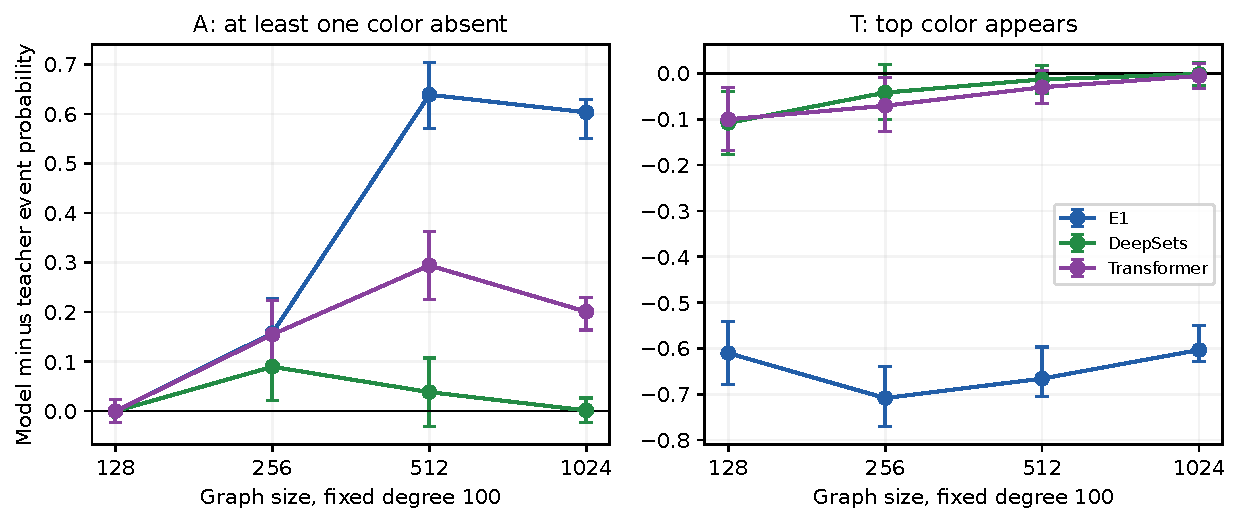
\includegraphics[keepaspectratio,alt={Fixed-cohort event-probability differences at degree 100, with simultaneous historical CP/Hoeffding bands. Curves concern two specific observables and do not order complete-law TV across graph sizes.}]{figures/integration-factorial.pdf}}
\caption{Fixed-cohort event-probability differences at degree 100, with
simultaneous historical CP/Hoeffding bands. Curves concern two specific
observables and do not order complete-law TV across graph sizes.}
\end{figure}

In regular graphs, degree also changes palette size. Their separate
causal effects are not identified by this design. Comparing TV lower
bounds on different graph spaces does not order the true TV values.
Three graph instances and five historical trainings constrain population
claims. The independent holdout witnesses and exploratory candidate
interventions remain separate analyses; an observed proposal/final-law
association is not alone a causal mediation result.

\section{What the baselines establish about
GNNs}\label{what-the-baselines-establish-about-gnns}

Neighborhood information has a precise role: free-color decisions
inspect fixed neighbors, and confirmation can require neighbors'
availability-dependent offers. The scoped indistinguishability examples
prove limits for an own-state or one-round current-state interface,
rather than proving that a large GNN is necessary for graph coloring.
Exact classical rules already solve the task with no trainable
parameters when their required information and schedule are supplied.

MAX provides a degree-insensitive representation of Boolean existence
and permits the finite-type COMMIT reduction. SUM can encode counts and
MEAN proportions; a training procedure may exploit
multiplicity-dependent shortcuts that fail outside the observed degrees.
The historical negative controls demonstrate such risks for specific
learned models. They do not constitute expressivity impossibility
results for those aggregators.

DeepSets and attention investigate how a node represents its palette.
Their success shows that the original prefix scorer is not the only
sufficient mechanism in the tested setting. Both still communicate over
graph edges. The small control tests reduced width within a normalized
family. The no-communication control tests missing information while
preserving core parameter count and supplied permissions. Any comparison
of those baselines must retain these differences.

The small LUBY model has 551 trainable parameters and completes all
1,280 LUBY evaluations; the small greedy control also completes all
1,280 under its supplied schedule. Thus the larger core is not
empirically necessary for those finite cells. In contrast, the
no-communication control completes 38/8,960 total attempts across the
seven teachers. This supports the value of received information under
this protocol, without proving that the particular large GNN or a
learned message MLP is necessary. Small-model failures for other
teachers are retained and do not establish incapacity beyond this
budget.

Teacher independence is similarly scoped. One architecture can expose
the action alphabet for all seven teachers, but supplied preferences,
priorities, phases and schedules change the observation interface.
Success across those interfaces is not learning arbitrary unseen
algorithms from identical raw inputs. The finite experiment supplies
evidence of adaptability, with cells that fail retained as limitations.

\section{How Much Supervision Does It Take to Learn a Distributed
Algorithm?}\label{how-much-supervision-does-it-take-to-learn-a-distributed-algorithm}

A teacher observation is one acquired decision label for a specified
node, state and action component. In ordinary color phases we count
participation, proposal and confirmation separately; Linial point
selection and speculative conflict marking each count as one. Replaying
a stored label adds optimizer work and no new supervision. Query counts,
component types, trajectory clusters, unique observations and data
hashes are recorded independently of updates. This distinction matters
because sequential imitation changes the states a policy visits
\citep{ross2010efficient, ross2011dagger}. Existing imitation
sample-complexity theory depends on its own state-space and horizon
assumptions \citep{rajaraman2020limits}; our finite curves imply no
analogous theoretical bound.

Information compatibility is established before comparing budgets.
Anonymous regime A contains LUBY, JOHANSSON and repeated COLOR\_TRIALS.
Extended regime B contains JP with explicit relative-ID comparisons, BE
with auxiliary colors, phase clock and supplied finite-field arithmetic,
GM with priority comparisons and its native block/repair schedule, and
sequential GREEDY with writable-node permissions. The three palette
architectures have identical teacher-specific observations and learned
graph messages. Transformer attention acts within a node's palette; it
is not a replacement for graph communication. Interface sufficiency
arguments and an anonymous-JP indistinguishability example do not prove
universal representability by these fixed network widths.

For a policy to PASS, every frozen execution must end with a proper
in-palette coloring, all protocol invariants respected, termination by
the teacher-specific deadline, and no technical error, cutoff or
incorrect terminal state. We use no 95\% functional threshold, repair
filter or failed-tape replacement. A teacher/architecture/budget
combination passes only when all five independently trained policies
pass their respective 1,000-case final batteries. These are five
separate policies, not one policy tested 5,000 times.

All seven exact teachers passed every frozen final case before student
confirmation. Native deadlines distinguish n-step sequential greedy and
JP's at-most-n priority steps from BE's 15 reductions and the randomized
teachers' prospective tail deadlines. Native steps with different
semantics are never directly interpreted as identical distributed
communication units.

The balanced cohort comprises 735 fresh trainings, five seeds per cell,
seven query budgets from 1,000 to 1,000,000, and 500 Adam updates per
training. Its shared teacher libraries acquired 34,999,967 component
labels in total; smaller-budget policies only access their hashed
prefixes. Training sizes are 8--24, development sizes 28/36, and
confirmation sizes 32/48/64, in seven prescribed graph strata. The first
budget where all five development policies are perfect nominates one
frozen candidate; final results cannot choose another budget. Of 21
teacher/architecture packages, 16 nominated a candidate, 12 achieved
five-seed PASS, and 80,000 final student executions were retained.

\textbf{Regime A. Smallest validated candidate budget, or explicit lack
of certification.}

{\def\LTcaptype{none} % do not increment counter
\begin{longtable}[]{@{}
  >{\raggedright\arraybackslash}p{(\linewidth - 6\tabcolsep) * \real{0.2500}}
  >{\raggedright\arraybackslash}p{(\linewidth - 6\tabcolsep) * \real{0.2500}}
  >{\raggedright\arraybackslash}p{(\linewidth - 6\tabcolsep) * \real{0.2500}}
  >{\raggedright\arraybackslash}p{(\linewidth - 6\tabcolsep) * \real{0.2500}}@{}}
\toprule\noalign{}
\begin{minipage}[b]{\linewidth}\raggedright
Teacher
\end{minipage} & \begin{minipage}[b]{\linewidth}\raggedright
E1: B*
\end{minipage} & \begin{minipage}[b]{\linewidth}\raggedright
DeepSets: B*
\end{minipage} & \begin{minipage}[b]{\linewidth}\raggedright
Transformer: B*
\end{minipage} \\
\midrule\noalign{}
\endhead
\bottomrule\noalign{}
\endlastfoot
LUBY & 1,000; 5/5 PASS & 3,000; 5/5 PASS & 1,000; 5/5 PASS \\
JOHANSSON & 1,000; 5/5 PASS & 1,000; 5/5 PASS & 1,000; 5/5 PASS \\
COLOR\_TRIALS & NOT CERTIFIED; 3/5 (candidate 300,000) & NOT CERTIFIED;
0/5 confirmed (no candidate; max 1,000,000) & NOT CERTIFIED; 0/5
confirmed (no candidate; max 1,000,000) \\
\end{longtable}
}

\textbf{Regime B. Smallest validated candidate budget, or explicit lack
of certification.}

{\def\LTcaptype{none} % do not increment counter
\begin{longtable}[]{@{}
  >{\raggedright\arraybackslash}p{(\linewidth - 6\tabcolsep) * \real{0.2500}}
  >{\raggedright\arraybackslash}p{(\linewidth - 6\tabcolsep) * \real{0.2500}}
  >{\raggedright\arraybackslash}p{(\linewidth - 6\tabcolsep) * \real{0.2500}}
  >{\raggedright\arraybackslash}p{(\linewidth - 6\tabcolsep) * \real{0.2500}}@{}}
\toprule\noalign{}
\begin{minipage}[b]{\linewidth}\raggedright
Teacher
\end{minipage} & \begin{minipage}[b]{\linewidth}\raggedright
E1: B*
\end{minipage} & \begin{minipage}[b]{\linewidth}\raggedright
DeepSets: B*
\end{minipage} & \begin{minipage}[b]{\linewidth}\raggedright
Transformer: B*
\end{minipage} \\
\midrule\noalign{}
\endhead
\bottomrule\noalign{}
\endlastfoot
JP & 1,000; 5/5 PASS & 1,000; 5/5 PASS & 1,000; 5/5 PASS \\
BE\_BASE\_D3 & NOT CERTIFIED; 0/5 confirmed (no candidate; max
1,000,000) & NOT CERTIFIED; 0/5 confirmed (no candidate; max 1,000,000)
& NOT CERTIFIED; 0/5 confirmed (no candidate; max 1,000,000) \\
SPECULATIVE\_GM & NOT CERTIFIED; 4/5 (candidate 30,000) & NOT CERTIFIED;
4/5 (candidate 30,000) & NOT CERTIFIED; 4/5 (candidate 30,000) \\
GREEDY & 1,000; 5/5 PASS & 1,000; 5/5 PASS & 1,000; 5/5 PASS \\
\end{longtable}
}

A NOT CERTIFIED cell reports an unachieved protocol threshold
B*\textgreater1,000,000, not an impossibility theorem. Its earlier
development budgets were evaluated; policies failing development were
not exhaustively tested in confirmation. Per-seed queries, failures,
compute and the distinction between an unattempted candidate and a
failed confirmation remain in the machine-readable tables.

\begin{figure}
\centering
\pandocbounded{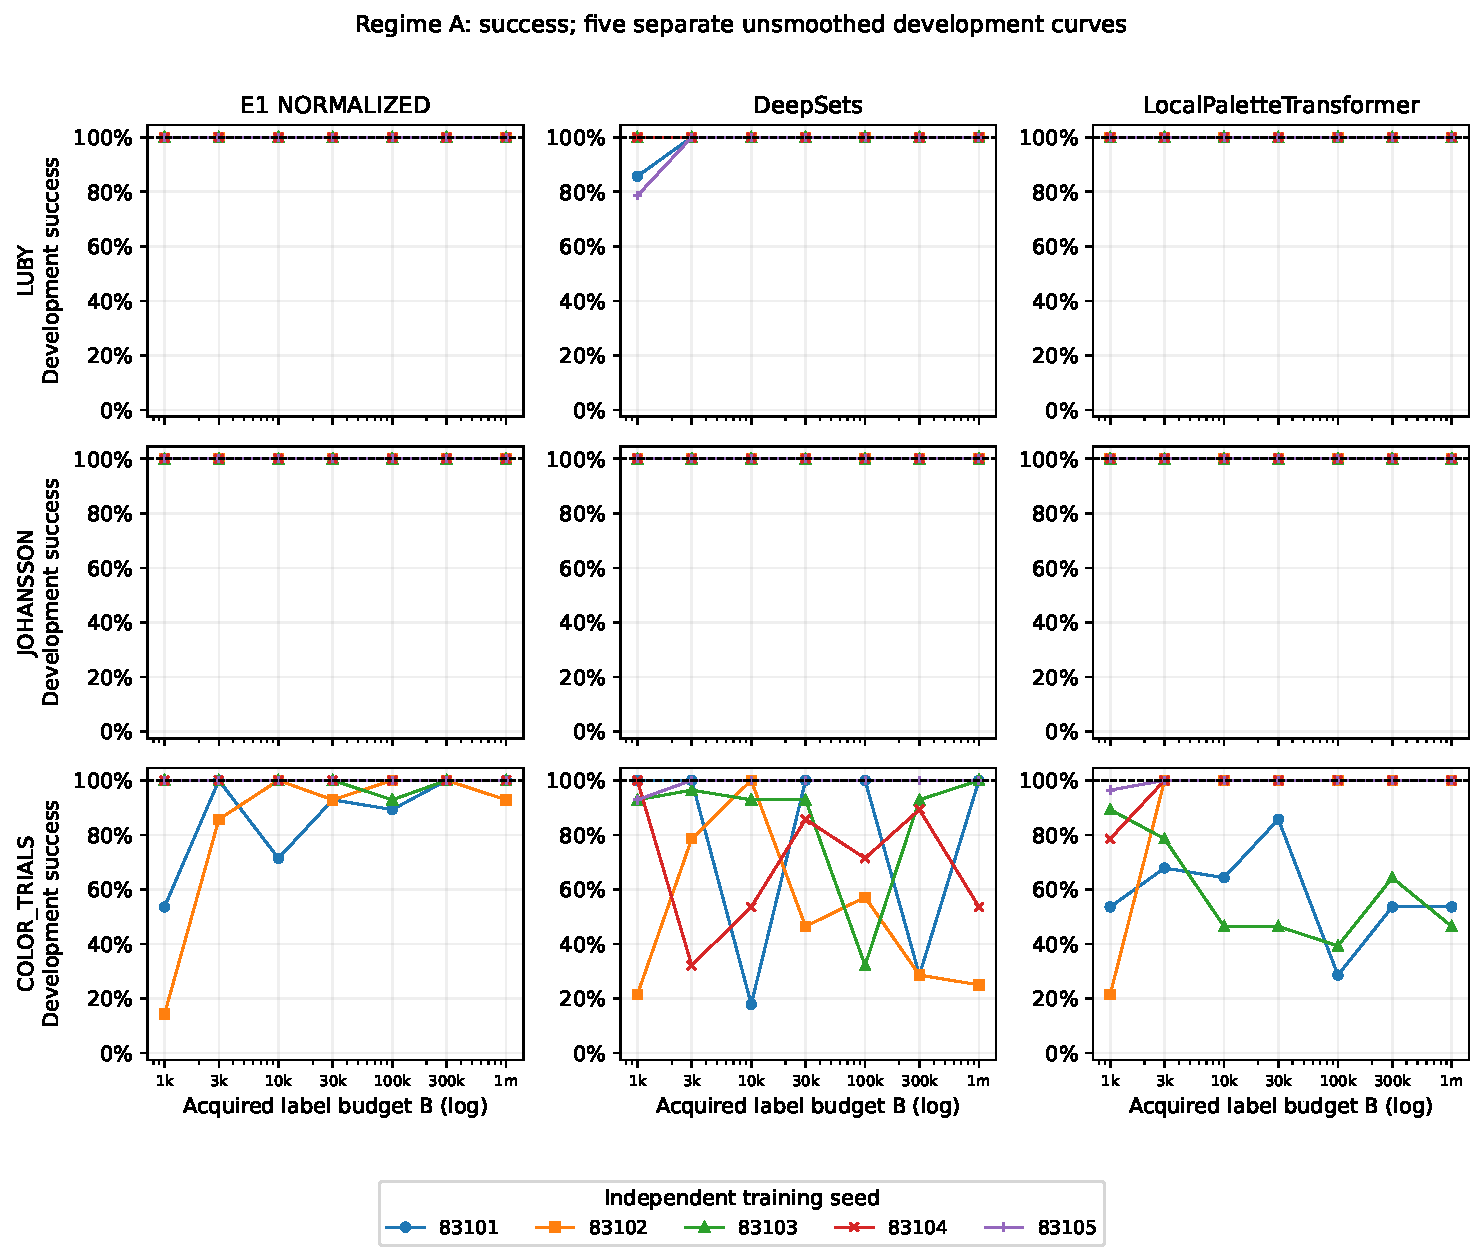
\includegraphics[keepaspectratio,alt={Anonymous-interface supervision curves. Each line is one training seed; these are development screens, not repeated final confirmations. The dashed line is the required 100\% frontier.}]{figures/sample-success-regime-a.pdf}}
\caption{Anonymous-interface supervision curves. Each line is one
training seed; these are development screens, not repeated final
confirmations. The dashed line is the required 100\% frontier.}
\end{figure}

\begin{figure}
\centering
\pandocbounded{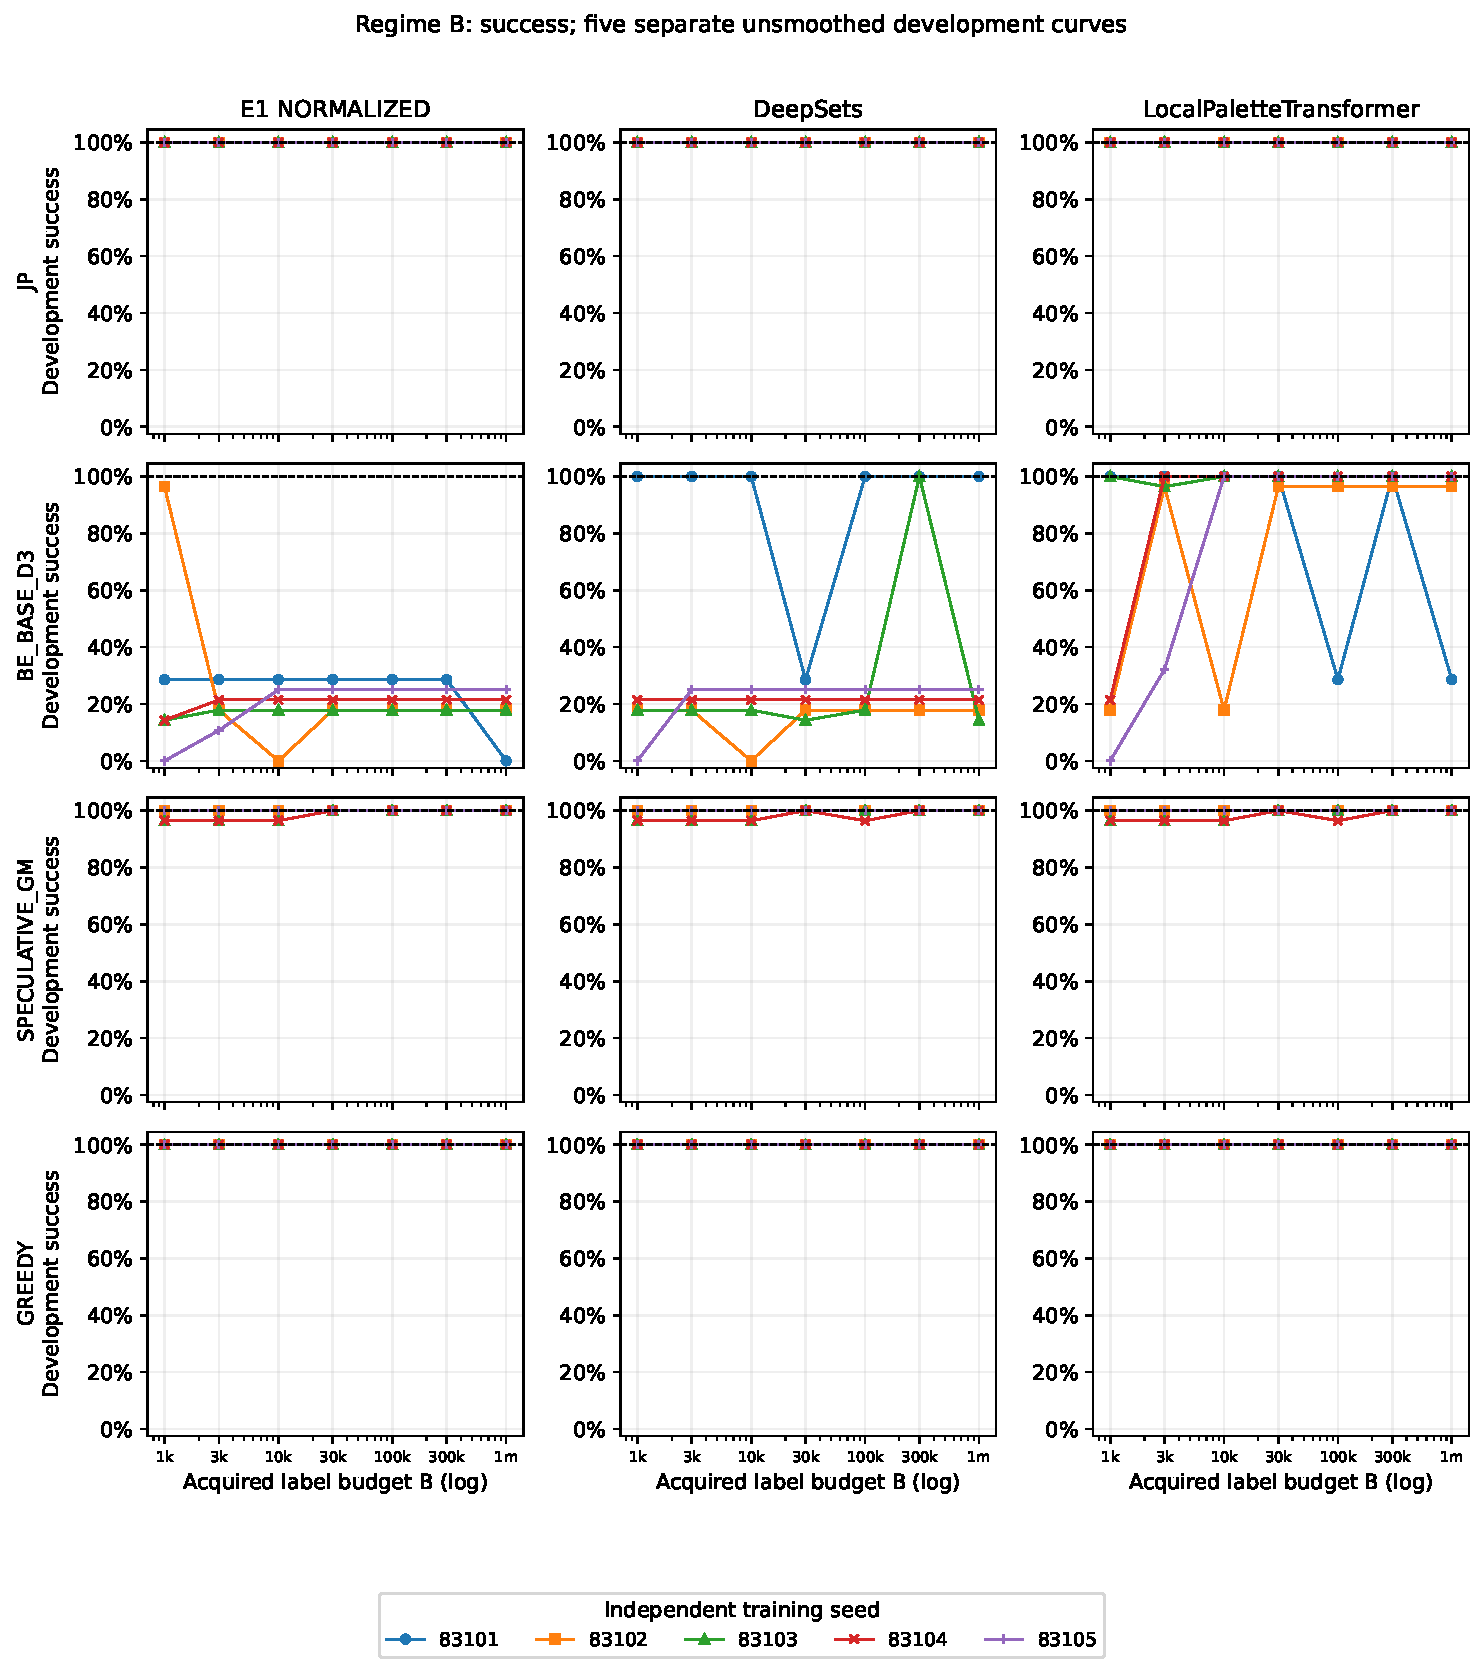
\includegraphics[keepaspectratio,alt={Extended-interface supervision curves with the same five-seed and 100\% rules. Declines are retained without smoothing.}]{figures/sample-success-regime-b.pdf}}
\caption{Extended-interface supervision curves with the same five-seed
and 100\% rules. Declines are retained without smoothing.}
\end{figure}

The grid does not assume monotonic improvement. Fixed optimization also
means larger libraries can leave more acquired observations unused;
visit counts are exported. Thus these are supervision curves conditional
on the specified optimizer budget, not pure information-theoretic sample
requirements.

For zero failures in 1,000 independent runs of one frozen policy, the
one-sided 95\% binomial lower success bound is 0.9970087504549047. Under
fixed independent strata the same zero-failure bound conservatively
controls their allocation-weighted mean by the arithmetic--geometric
mean inequality. It does not cover every graph or simultaneously all
trained policies. The five seeds remain the units of training
replication.

\subsection{Optimization, capacity and interactive
controls}\label{optimization-capacity-and-interactive-controls}

The following entries count seeds completing all development cases, at
the same B=3,000. They are exploratory development outcomes, never final
PASS:

{\def\LTcaptype{none} % do not increment counter
\begin{longtable}[]{@{}
  >{\raggedright\arraybackslash}p{(\linewidth - 10\tabcolsep) * \real{0.1667}}
  >{\raggedright\arraybackslash}p{(\linewidth - 10\tabcolsep) * \real{0.1667}}
  >{\raggedright\arraybackslash}p{(\linewidth - 10\tabcolsep) * \real{0.1667}}
  >{\raggedright\arraybackslash}p{(\linewidth - 10\tabcolsep) * \real{0.1667}}
  >{\raggedright\arraybackslash}p{(\linewidth - 10\tabcolsep) * \real{0.1667}}
  >{\raggedright\arraybackslash}p{(\linewidth - 10\tabcolsep) * \real{0.1667}}@{}}
\toprule\noalign{}
\begin{minipage}[b]{\linewidth}\raggedright
Teacher
\end{minipage} & \begin{minipage}[b]{\linewidth}\raggedright
Passive E1 500 updates
\end{minipage} & \begin{minipage}[b]{\linewidth}\raggedright
Passive E1 1,500 updates
\end{minipage} & \begin{minipage}[b]{\linewidth}\raggedright
Small 500
\end{minipage} & \begin{minipage}[b]{\linewidth}\raggedright
No messages 500
\end{minipage} & \begin{minipage}[b]{\linewidth}\raggedright
Interactive 500 total
\end{minipage} \\
\midrule\noalign{}
\endhead
\bottomrule\noalign{}
\endlastfoot
LUBY & 5/5 & 5/5 & 1/5 & 0/5 & 4/5 \\
JP & 5/5 & 5/5 & 0/5 & 0/5 & 5/5 \\
BE (D3) & 0/5 & 5/5 & 0/5 & 0/5 & 1/5 \\
\end{longtable}
}

The fixed-label control changes only E1's optimizer updates. The small
and no-message models share the same label prefix and update budget. The
one-aggregation interactive control allocates half the labels to passive
warmup and half to admissible states visited by the warm policy, with
250+250 updates and an Adam reset at aggregation. Failed learner
trajectories remain recorded. It excludes GM's unproved
arbitrary-history interface. These limited controls cannot identify
every failure as a representation or data limitation.

Functional PASS does not logically imply action or transition fidelity,
teacher-like execution time, or equality of complete coloring laws.
Separate teacher-state fidelity and native-step curves retain all five
seeds. Historical law tests are not imported as evidence for the new
checkpoints. The full protocol, audit, negative results,
dataset/checkpoint hashes and reproducible figure sources accompany this
finite empirical statement.

The GM confirmation failures (normalized: 79, deepsets: 79, transformer:
79) leave only isolated vertices uncolored and occur in training seed(s)
83105. A post hoc singleton witness using the frozen candidate weights
reproduces an incorrect confirmation rejecting assignment despite
positive participation, while the exact teacher succeeds. The cached
prefix contains 5 isolated-assignment bundles (three component labels
per bundle), and the exact recorded minibatch order presents them 9
times; the affected seed's development suite contains 0 isolated
vertices. This identifies a rare-state fit defect missed by development
coverage. It does not show an absence of ID information or prove a
universal capacity limitation. The diagnostic changes no model, budget,
primary classification or final tape. Full traces and presentation-count
checks are in structural-failure-witnesses.json.

The independent exploratory coloring-law supplement tests 210 fixed
teacher/checkpoint/graph hypotheses using the audited native K4 robust
instrument, split selection/evaluation rows, 9,999 permutations and Holm
over the complete family. 210 comparisons are testable and 0 reject.
Untestable comparisons retain p=1; conservative futility also cannot
create rejection. These are conditional-on-success laws on two fixed
small graphs, not equality guarantees or an additional functional PASS
condition.

The small-model supplement repeats all seven budgets for three
representative teachers and freezes independent final tapes under the
same five-seed gate:

{\def\LTcaptype{none} % do not increment counter
\begin{longtable}[]{@{}
  >{\raggedright\arraybackslash}p{(\linewidth - 8\tabcolsep) * \real{0.2000}}
  >{\raggedright\arraybackslash}p{(\linewidth - 8\tabcolsep) * \real{0.2000}}
  >{\raggedright\arraybackslash}p{(\linewidth - 8\tabcolsep) * \real{0.2000}}
  >{\raggedright\arraybackslash}p{(\linewidth - 8\tabcolsep) * \real{0.2000}}
  >{\raggedright\arraybackslash}p{(\linewidth - 8\tabcolsep) * \real{0.2000}}@{}}
\toprule\noalign{}
\begin{minipage}[b]{\linewidth}\raggedright
Teacher
\end{minipage} & \begin{minipage}[b]{\linewidth}\raggedright
Small parameters
\end{minipage} & \begin{minipage}[b]{\linewidth}\raggedright
Small validated B*
\end{minipage} & \begin{minipage}[b]{\linewidth}\raggedright
Seeds confirmed
\end{minipage} & \begin{minipage}[b]{\linewidth}\raggedright
Final attempted
\end{minipage} \\
\midrule\noalign{}
\endhead
\bottomrule\noalign{}
\endlastfoot
LUBY & 551 & NOT CERTIFIED & 0/5 & False \\
JP & 1560 & NOT CERTIFIED & 0/5 & False \\
BE\_BASE\_D3 & 1560 & NOT CERTIFIED & 0/5 & False \\
\end{longtable}
}

Without a common development candidate no student final is attempted.
These outcomes establish neither universal minimality nor the behavior
of all possible small networks.

The additional fixed-label optimization protocol freezes both existing
optimizer arms for all three control teachers and evaluates them on new
paired final batteries. It checks identical label-prefix and
initialization hashes and changes no primary outcome:

{\def\LTcaptype{none} % do not increment counter
\begin{longtable}[]{@{}lll@{}}
\toprule\noalign{}
Teacher & 500 updates, B=3,000 & 1,500 updates, B=3,000 \\
\midrule\noalign{}
\endhead
\bottomrule\noalign{}
\endlastfoot
LUBY & PASS (5/5) & PASS (5/5) \\
JP & PASS (5/5) & PASS (5/5) \\
BE\_BASE\_D3 & NOT CERTIFIED (0/5) & PASS (5/5) \\
\end{longtable}
}

A PASS here validates the fixed B=3,000/optimizer point only; it is not
a new grid minimum or a retry of the primary confirmation.

\section{Discussion}\label{discussion}

The evidence supports the proposed distinction among notions of
learning. The native JP example separates local action accuracy from
autonomous validity. The historical palette study separates successful
coloring from exact candidate imitation. Full-law tests and event bounds
separate task validity from teacher-distribution fidelity. Clique
symmetry and scoped coupling certificates show why the converse
statement, that every imitating network must have a different global
law, would also be false.

Teacher changes can affect a policy without changing its unrestricted
output law. Exact synchronous JP with fixed distinct priorities gives
the same first-fit solution as sequential greedy in descending priority
order. If ID order is uniform, ascending and descending orders are both
uniform, so uncapped JP and random-order greedy induce the same
final-coloring law. Their common-ID executions and native costs can
differ. Conditioning JP on a restrictive 128-round cap can also change
that equality. This elementary observation prevents equating algorithm
identity with solution-law identity.

The statistical reconciliation illustrates a complementary point. A
characteristic kernel identifies laws in the population but can place a
large TV difference in a weak finite-sample direction. Honest local
witness selection can help in a specified alternative class while
preserving conditional calibration. It can still miss rare or
unrepresented high-order effects. Statistical instruments are part of
the experiment, not neutral or universally powerful labels attached
afterwards.

The strongest paper narrative therefore concerns the relationship
between teacher specification, architectural information and the notion
of fidelity. It does not require deciding that one research line was
right and the other wrong. Differences caused by definitions should be
stated; actual bugs should be repaired with evidence; remaining
numerical gaps should remain open. This approach permits a defensible
joint interpretation without erasing contradictory-looking historical
records.

\section{Limitations and unresolved
claims}\label{limitations-and-unresolved-claims}

The principal historical limitation is missing collaborator runtime
data: five retrained E1s,35 native E1s, source pools and original full
coloring banks. Published tables and sources can be checked, but exact
model-level reproduction has not been completed. The new 70-model cohort
is not a substitute for those artifacts. Independent scientific review
of this integrated draft remains pending.

The historical balanced integration design has two initialization
replicas,24 training graphs, one trajectory per graph and a much smaller
exposure budget than the earlier full-budget studies. It does not
identify an asymptotic architecture ranking or separate optimization
from capacity in failed cells. Native teacher generalization above
degree 3 or to local palettes is unsupported by this interface. The
separate historical local-palette evidence must retain its own
checkpoints and protocols.

The separate supervision study uses five replicas and controlled
acquired-label budgets but only 500 primary updates and a finite
graph/tape distribution. Its additional fixed-label optimization and
interactive controls probe selected failure mechanisms; they do not
identify an intrinsic information-theoretic sample requirement or
establish a universal architecture ranking. Its local prospective freeze
is not an independently timestamped external registration.

Finite functional success does not prove universal neural safety,
termination or complexity preservation. Canonical MAX certificates
require precise algebraic/numerical assumptions and do not cover every
native context head. The simulator is synchronous, with supplied
schedules and arithmetic for some teachers; distributed preprocessing
and asynchronous deployment are not evaluated.

Output-law tests have finite power and resolution. Their nonrejections
are not equality statements, while conditional solution laws do not
determine failure or stopping-time laws. Multiple separate historical
families do not give one 5\% guarantee over their union.
CP/Hoeffding/DKW bounds concern their stated finite cohort or observable
families, not a graph population. No causal degree/palette separation or
general monotone TV law is established.

\section{Counterfactual supervision across native
teachers}\label{counterfactual-supervision-across-native-teachers}

\subsection{Reconstruction and causal
domains}\label{reconstruction-and-causal-domains}

We reconstruct M6B from authenticated original source and 21 historical
artifacts. The 249/500 traditional, 476/500 own-proposal and 500/500
counterfactual outcomes concern one training seed, 10001, on paired
cubic N10240 cases. Thirty original-policy executions are replayed
exactly. M6B uses the 8967-parameter M4B architecture, whereas canonical
E1 has 16035 parameters. The own/CF checkpoints share every
participation, first-message and candidate tensor; only the
second-message and COMMIT tensors differ. The configured 120-epoch
horizon is 17760 updates; the selected checkpoints are epoch 53, or 7844
updates. The traditional comparison also changes the number of tapes per
graph, so its improvement is not a pure CF effect.

Pedro's 16 source hashes are verified against commits fc756cef, 80f486eb
and 6836d855. None of the 40 expected original E1 weight hashes was
recovered from 6614 local checkpoint files or the inspected public
release manifests. His five 1980/1980 results, JP 1631/1980 and GM
1951/1980 remain authenticated reported evidence with five
initializations over 396 published cases and a common training pool. His
17760 updates of 1680 roots and own/CF training also differ from the
primary 500-update, batch 64 passive study. New runs below reproduce
mechanisms, not those unavailable original policies.

We define a phase-specific label operation

\[\mathcal O_T(S,a,\xi)=D_T^\phi\bigl(R_T^\phi(S,a,\xi)\bigr),\]

where \(S\) is an admissible native snapshot, \(a\) a typed
intervention, \(\xi\) the private input, and \(R\) recomputes every
causal descendant before the phase decision \(D\) is queried. We
distinguish native decisions from defensive continuation queries on
offers that the native policy might not emit. The latter are additional
supervised tasks, not a claim that arbitrary simulator arrays are
reachable teacher states. For BE and JP, forced participation cannot
bypass phase eligibility or priority; ColorTrials confirmation requires
strict winning preferences under actual availability. Linial points and
GM detection marks have separate native oracles.

Admissible contexts are reconstructed from legal prefixes. Changing IDs
requires a new complete replay, including comparisons, blocks,
permissions and auxiliary initial colors. Private preference/draw
interventions preserve the persistent state and regenerate messages. KW
arithmetic and Linial evaluations are recomputed; speculative GM
histories retain their supplied schedule, actual assignment colors,
marks and repair queue. We export 162 additional hard contexts with
replay witnesses. The three palette cores share these training-only
adapters. All teacher and autonomous inference source files remain
unchanged from the baseline; no exact decision replaces the neural
confirmation head.

\subsection{Paired controls and strict new
certifications}\label{paired-controls-and-strict-new-certifications}

We train 135 primary runs: three pending teachers, three cores, five new
seeds and three treatments. Each preserves 500/1500/4000 checkpoints,
the same native bank, initialization and minibatch sequence within a
seed/core. Passive is the historical loss. Matched evaluates COMMIT with
its stored teacher proposals and corresponding label. Fixed-bank CF uses
100 matched warmup updates, then P + C + .5 matched confirmation + .5 CF
confirmation. Each normal root acquires three native component labels
and four additional stored confirmation queries; Linial and DETECT each
acquire one native label. Own-proposal queries in a separate
seven-teacher pilot are charged individually.

Training uses N8/12/16/24. An amendment recorded before the additional
screen and all new finals expands development from 60 to 300 cases at
N28/36. The first common perfect checkpoint is frozen per treatment.
Final has five independent 1000-case batteries at N32/48/64, ten fixed
family strata, native horizons, and the strict original
invariant/terminal gate.

Matched passes all nine pending packages, using 1500 updates for BE, 500
for ColorTrials/E1, 1500 for its other cores and 500 for GM. CF
initially fails BE at 1500 in seed 94105 for all cores, and
ColorTrials/E1 at 500 in seed 94103. Independently frozen follow-ups
compare existing 1500/4000 CF checkpoints on new namespaces, retaining
both outcomes. BE 1500 again fails in seed 94105;
ColorTrials/Transformer1500 has two failures in its new battery. All six
4000-update packages pass. The following CF fixed points therefore close
all nine cells, while the historical twelve remain separate: coverage is
21/21, not one homogeneous newly retrained cohort.

{\def\LTcaptype{none} % do not increment counter
\begin{longtable}[]{@{}llllll@{}}
\toprule\noalign{}
Teacher & Core & Updates & Native labels & All labels & Final \\
\midrule\noalign{}
\endhead
\bottomrule\noalign{}
\endlastfoot
BE & normalized & 4000 & 3000 & 6776 & 5 x 1000/1000 \\
BE & deepsets & 4000 & 3000 & 6776 & 5 x 1000/1000 \\
BE & transformer & 4000 & 3000 & 6776 & 5 x 1000/1000 \\
ColorTrials & normalized & 4000 & 30000 & 70000 & 5 x 1000/1000 \\
ColorTrials & deepsets & 4000 & 30000 & 70000 & 5 x 1000/1000 \\
ColorTrials & transformer & 4000 & 30000 & 70000 & 5 x 1000/1000 \\
GM & normalized & 500 & 3000 & 6104--6120 & 5 x 1000/1000 \\
GM & deepsets & 500 & 3000 & 6104--6120 & 5 x 1000/1000 \\
GM & transformer & 500 & 3000 & 6104--6120 & 5 x 1000/1000 \\
\end{longtable}
}

The complete extension retains 195000 final execution rows, 194979
correct, and 170 distinct frozen checkpoints. Repeated checkpoints on a
second battery are not new training replicas. All eight representative
failed checkpoint/battery traces reproduce their original outcomes under
the same 32-case cohort and 1024-root numerical batching. BE failures
are omitted required KW recolorings that violate the new auxiliary
bound. No failure is repaired or removed. An explicit erratum preserves
and corrects the CT follow-up plan's reason-text typo (the original E1
failure was at 500, not1500); the actual checkpoint hashes, batteries
and rows are unchanged.

\begin{figure}
\centering
\pandocbounded{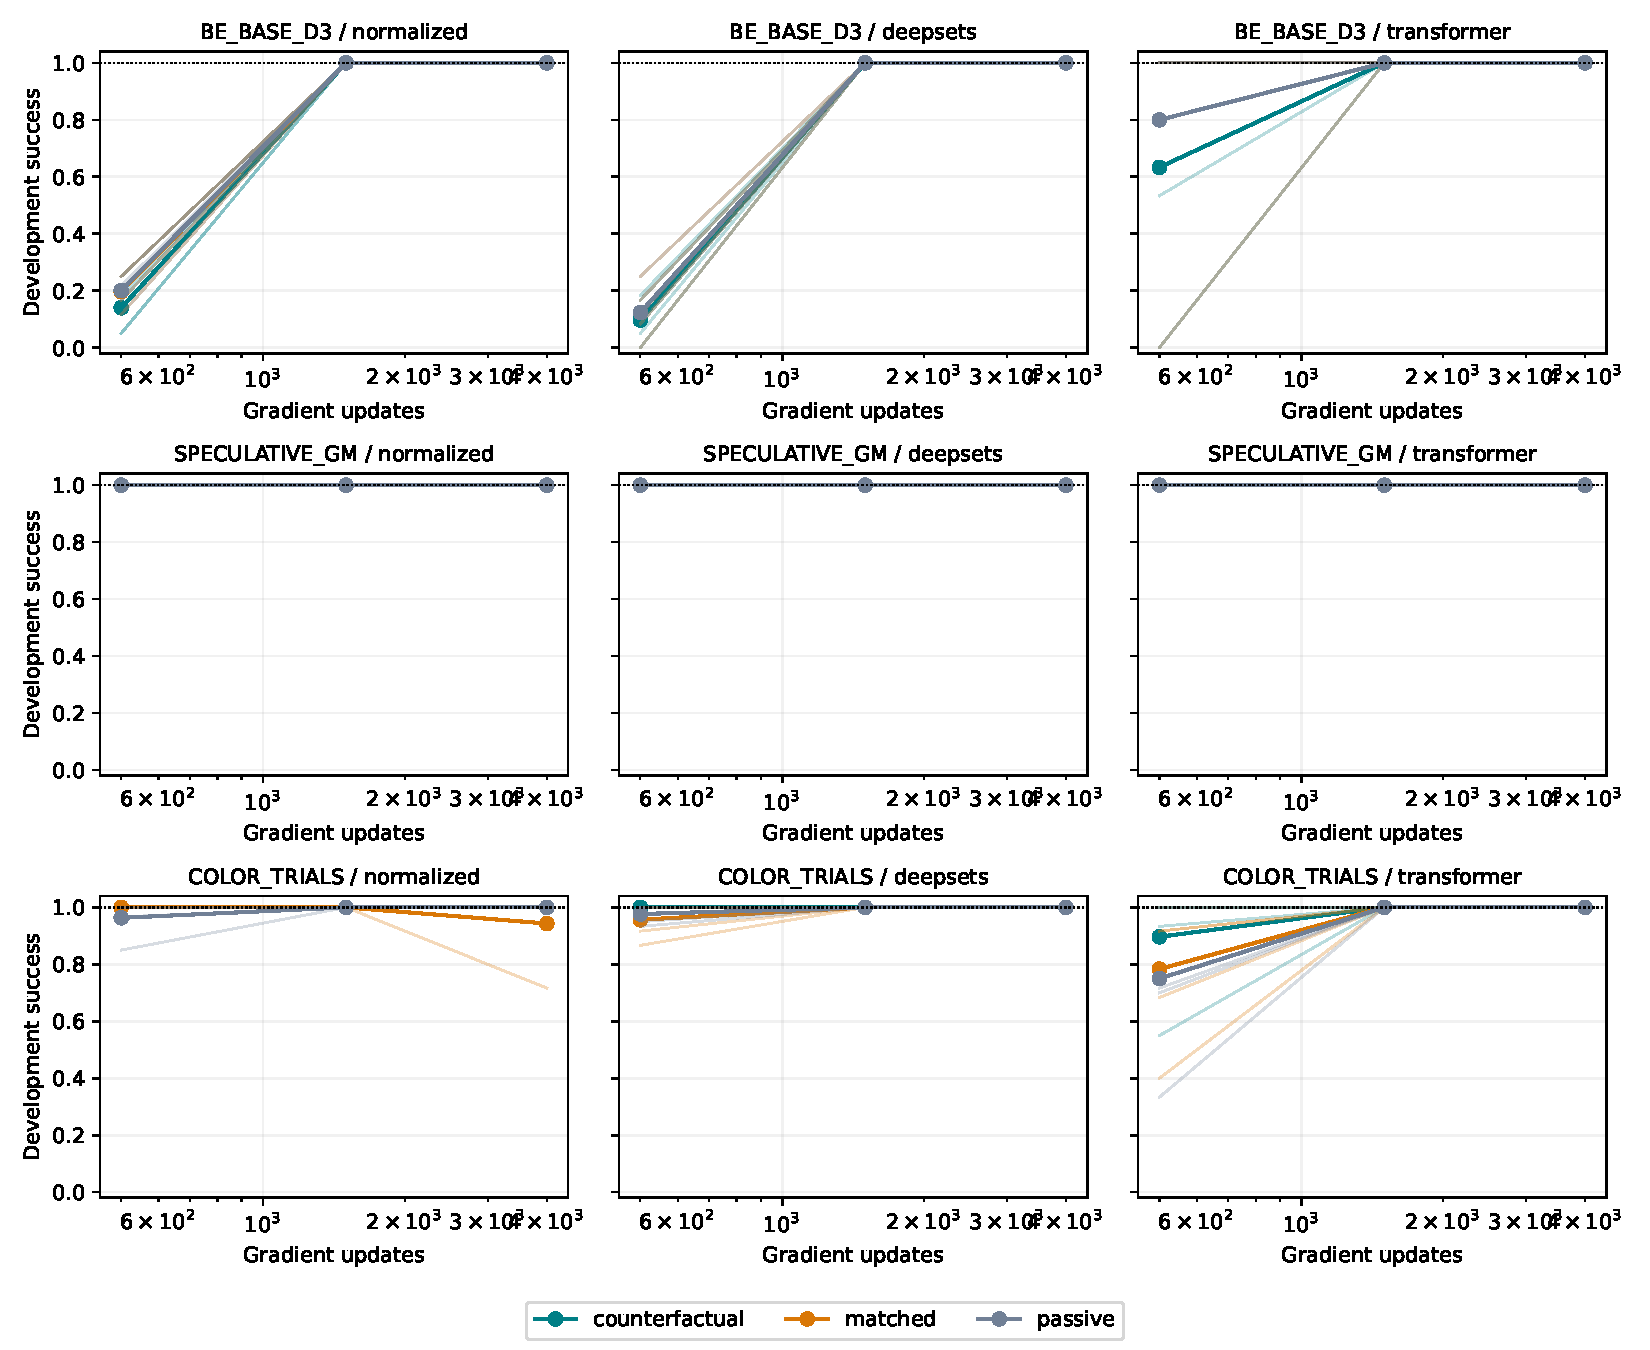
\includegraphics[keepaspectratio,alt={All five unsmoothed development curves and descriptive means at fixed native banks. Perfect development is a selection screen, not a functional certificate.}]{figures/multicf-optimization-curves.pdf}}
\caption{All five unsmoothed development curves and descriptive means at
fixed native banks. Perfect development is a selection screen, not a
functional certificate.}
\end{figure}

\subsection{Functional validity and continuation
fidelity}\label{functional-validity-and-continuation-fidelity}

At 4000, all permitted roots in 60 common native development
trajectories per seed are audited, with four fresh continuation queries
per color root. The table reports descriptive aggregate percentages
across five policies; root decisions are not independent training
replicas. Per core, the CF denominators are 499200 for BE, 41036 for GM
and 57576 for ColorTrials. Full per-seed action, actual-transition,
component and phase counts remain machine-readable. The certified GM500
policies have separate full audits at their actual checkpoint; the table
fixes4000 for the paired comparison. CF improves the broader
continuation task, while the matched/passive procedures already satisfy
the functional gate. Thus CF is not uniformly necessary, or better at
the same update count, for native functional success. A matched
ColorTrials/E1 run regresses from 60/60 to 43/60 development successes
between 1500 and4000 updates.

{\def\LTcaptype{none} % do not increment counter
\begin{longtable}[]{@{}
  >{\raggedright\arraybackslash}p{(\linewidth - 8\tabcolsep) * \real{0.2000}}
  >{\raggedright\arraybackslash}p{(\linewidth - 8\tabcolsep) * \real{0.2000}}
  >{\raggedright\arraybackslash}p{(\linewidth - 8\tabcolsep) * \real{0.2000}}
  >{\raggedright\arraybackslash}p{(\linewidth - 8\tabcolsep) * \real{0.2000}}
  >{\raggedright\arraybackslash}p{(\linewidth - 8\tabcolsep) * \real{0.2000}}@{}}
\toprule\noalign{}
\begin{minipage}[b]{\linewidth}\raggedright
Teacher
\end{minipage} & \begin{minipage}[b]{\linewidth}\raggedright
Core
\end{minipage} & \begin{minipage}[b]{\linewidth}\raggedright
Matched CF (\%)
\end{minipage} & \begin{minipage}[b]{\linewidth}\raggedright
CF-trained CF (\%)
\end{minipage} & \begin{minipage}[b]{\linewidth}\raggedright
CF native actions (\%)
\end{minipage} \\
\midrule\noalign{}
\endhead
\bottomrule\noalign{}
\endlastfoot
BE & normalized & 9.269 & 99.993 & 100.000 \\
BE & deepsets & 9.269 & 99.993 & 100.000 \\
BE & transformer & 9.269 & 99.993 & 100.000 \\
GM & normalized & 75.363 & 100.000 & 100.000 \\
GM & deepsets & 75.363 & 100.000 & 100.000 \\
GM & transformer & 75.363 & 100.000 & 99.995 \\
ColorTrials & normalized & 97.256 & 99.745 & 99.187 \\
ColorTrials & deepsets & 99.097 & 100.000 & 100.000 \\
ColorTrials & transformer & 98.076 & 100.000 & 100.000 \\
\end{longtable}
}

For BE/GM, every second-stage and COMMIT tensor is identical across the
three palette cores in each paired fixed-proposal seed/update
comparison. Those losses do not use the candidate scorer, whereas
ColorTrials reads its candidate after the second exchange and couples
those gradients. Shared heads explain correlated architecture outcomes;
they do not provide three independent confirmations of a head-level
effect.

\begin{figure}
\centering
\pandocbounded{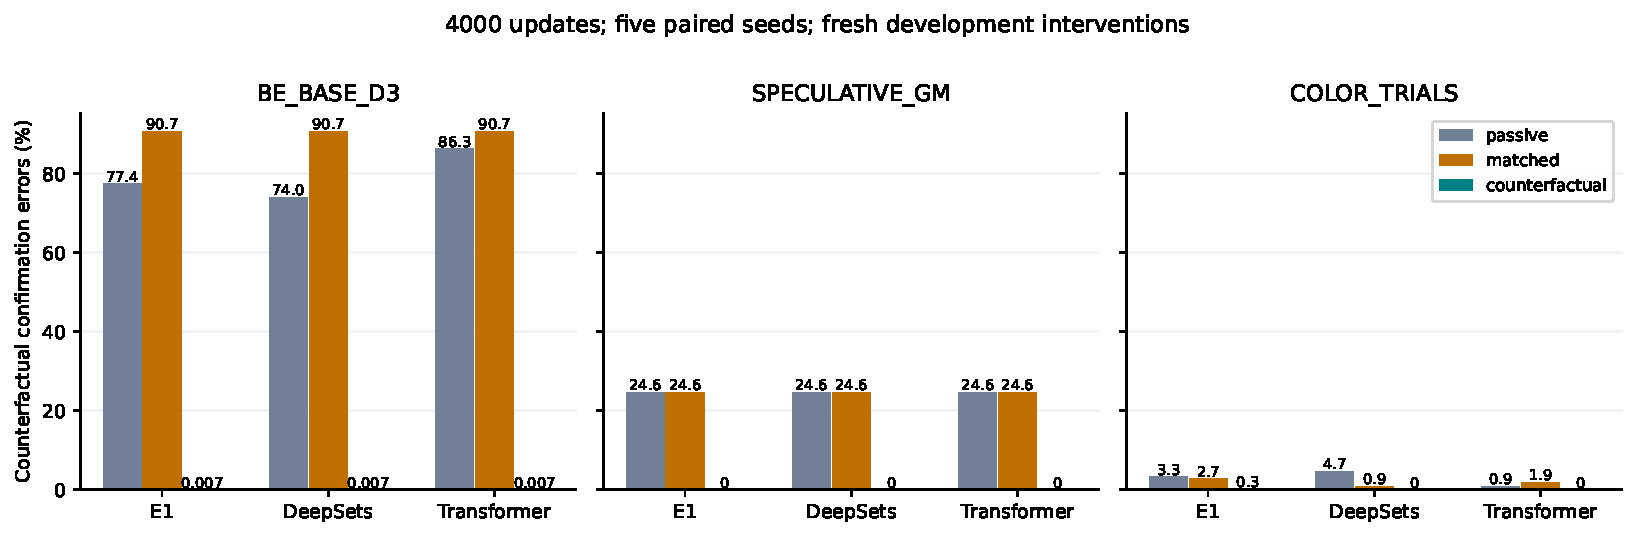
\includegraphics[keepaspectratio,alt={Errors on fresh continuation queries, separated from native action fidelity. Small nonzero errors retain explicit labels.}]{figures/multicf-counterfactual-fidelity.pdf}}
\caption{Errors on fresh continuation queries, separated from native
action fidelity. Small nonzero errors retain explicit labels.}
\end{figure}

Nested ColorTrials banks at native budgets 1000/3000/10000/30000 and
fixed 500/1500 updates provide development-only supervision curves.
Every CF label is charged; these do not establish a new certified
minimum. A matched GM control without the added isolate families also
passes all five new development seeds, so the tested ablation does not
isolate a positive coverage effect. The authenticated old seed 83105
failures and all 30 new regressions remain a separate observation. The
own-plus-CF portability pilot passes 60/60 development in six teachers
for one new E1 seed, but BE obtains 22/60 at 1500; copying the Luby
curriculum is insufficient evidence of a uniformly successful
multiteacher procedure.

\begin{figure}
\centering
\pandocbounded{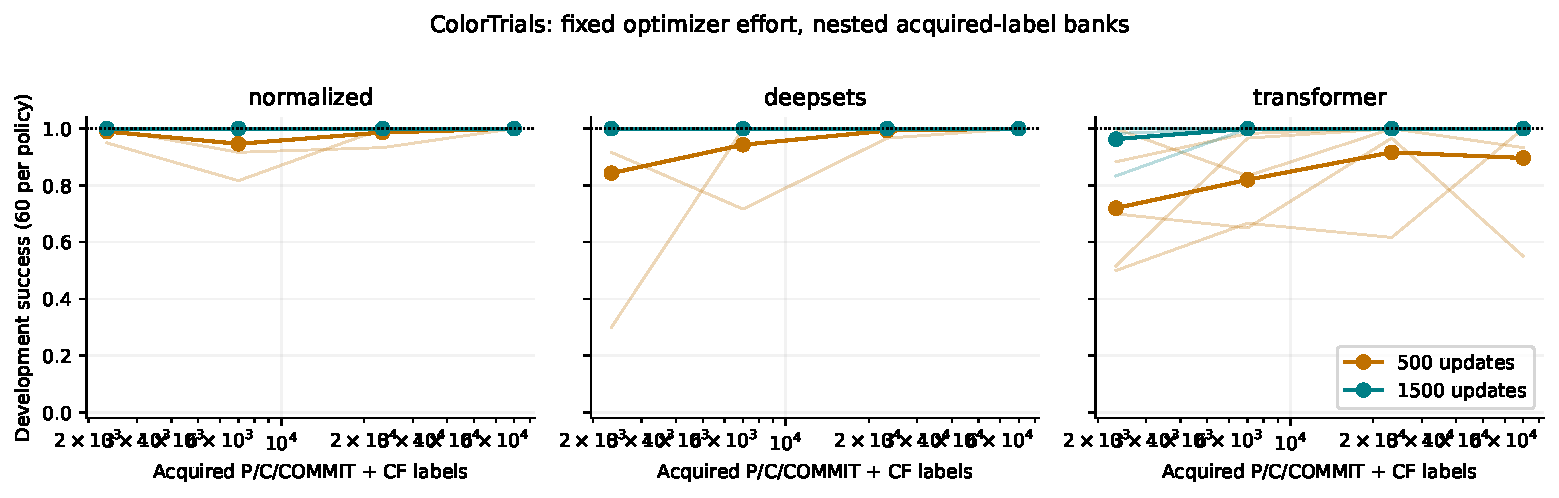
\includegraphics[keepaspectratio,alt={Supervision and optimization are distinct axes; thin lines show all five seeds. These lower-budget points have no new final certification.}]{figures/multicf-supervision-curves.pdf}}
\caption{Supervision and optimization are distinct axes; thin lines show
all five seeds. These lower-budget points have no new final
certification.}
\end{figure}

\subsection{Information, complete outputs and
transfer}\label{information-complete-outputs-and-transfer}

JP's information control fixes the architecture, labels, batches, 500
updates and initialization, changing only two local context channels.
Relative order passes all five 60-case development suites; raw endpoint
IDs, differences and removed IDs do not. Twenty numerical replays
reproduce every original ablation weight tensor and retain intermediate
Adam/RNG checkpoints.

{\def\LTcaptype{none} % do not increment counter
\begin{longtable}[]{@{}ll@{}}
\toprule\noalign{}
JP representation & Development successes, five seeds (/60) \\
\midrule\noalign{}
\endhead
\bottomrule\noalign{}
\endlastfoot
without\_ids & 6, 6, 6, 6, 6 \\
numeric\_ids & 13, 11, 6, 26, 15 \\
numeric\_differences & 16, 15, 19, 31, 20 \\
relative\_comparisons & 60, 60, 60, 60, 60 \\
\end{longtable}
}

An indistinguishability witness swaps the IDs on a pending edge:
anonymous observations are equal but native eligibility reverses. Edge
order suffices for the implemented priority decision. This is an
observation-level obstruction, not a claim that numeric IDs are
unlearnable. ColorTrials has a second-hop availability witness.
Historical M6 also aliases the float64 draws \(1/2-2^{-28}\) and
\(1/2+2^{-28}\) to the same float32 observation, despite opposite
activation labels. The current native teacher directly queries its
supplied float32 inputs, avoiding that particular obstruction.

\begin{figure}
\centering
\pandocbounded{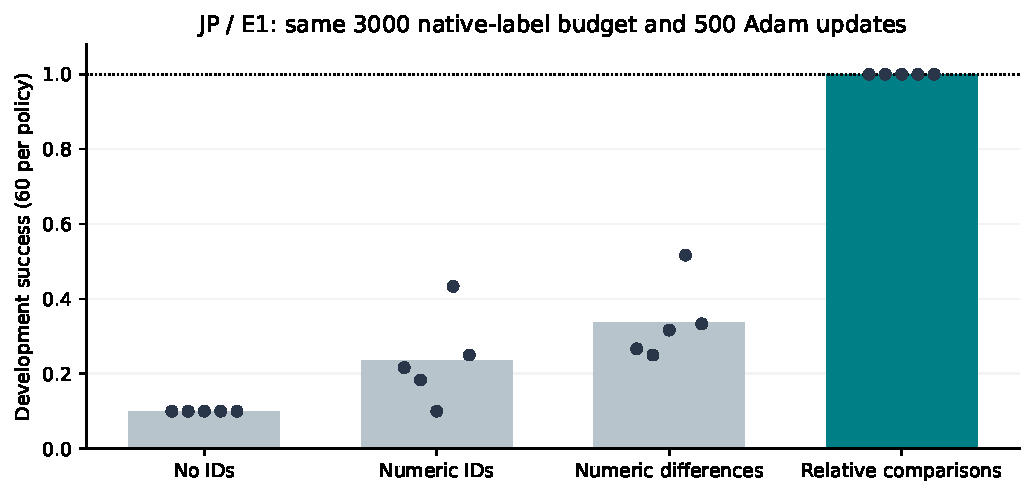
\includegraphics[keepaspectratio,alt={Information representation at a fixed optimizer and label point. Each dot is one training seed; development performance is not final certification.}]{figures/multicf-jp-information.pdf}}
\caption{Information representation at a fixed optimizer and label
point. Each dot is one training seed; development performance is not
final certification.}
\end{figure}

After functional selection, all 45 successful CF policies are frozen
before fresh law and transfer tapes. On path8 and K4 plus four isolates,
256 shared-input runs per graph/policy compare the full labelled
terminal vector and status, without success filtering. The coupling
inequality and exact one-sided binomial bounds with Bonferroni .05/90
yield 89/90 simultaneous TV-at-most-.05 certificates. These are
approximate fixed-graph marginal-law bounds, not equality.
ColorTrials/E1 seed 94104 on path8 has36/256 coupled disagreements,
upper bound .223630 and mean 2.191406 native steps versus 2.097656.
Coupled disagreement is not a TV lower bound or proof that the marginal
laws differ. Empirical full-vector histograms and native times are
retained separately.

Exploratory transfer obtains 3780/3780 correct executions, 84 per policy
at N128/256/512. Its ten domain families are supplemented by binary
trees, diamond chains, triangle chains and subdivided K4 components, all
of maximum degree3. These finite observations do not extend the teacher
to higher degree, local palettes or arbitrary graphs/tapes. Functional
validity does not establish universal decision or law identity.

The complete campaign contains 278 computational training runs,
including paired arms, pilots and numerical replays, with 683504
gradient updates and 2.580 CPU optimization hours. Training GPU time is
zero; the original M6 CUDA replay is separate. Process times overlap.
Acquired components, reused labels, presentations, simulator work and
optimization remain separate; no sample-efficiency claim compares
unequal update budgets. All sources, models, datasets, witnesses,
negative results and manifests accompany this extension. The
verification recomputes every final gate and all stored CF labels with
zero label inconsistencies. The full suite's639 cases and29 later added
cases pass.

These contributions complement trace-oriented CLRS
\citet{velickovic2022clrs} and learner-state acquisition in DAgger
\citet{ross2011dagger}. Recent contrastive graph-coloring work
\citet{le2026contrastive} studies approximate-coloring objectives. Our
contribution is the specified admissible-oracle framework, controlled
separation of training factors, and finite native execution evidence; no
comprehensive bibliographic priority or universal learnability claim
follows from this study.


\section{Conclusions}\label{conclusions}

Learning from an algorithmic teacher has several distinct targets. Our
integrated coloring project shows how the teacher's information and
action interface constrain architecture design, how strong local
imitation can fail in autonomous execution, and how functional
extrapolation can coexist with a changed complete-solution law. Exact
teacher baselines and smaller controls prevent attributing classical
task solvability to GNN complexity alone. Symmetry and coupling also
identify settings where distributional agreement is possible despite
different decision mechanisms.

The counterfactual extension supplies independently validated functional
points for all nine pending packages, preserving the prior twelve as
historical reference. Its controls show that label concordance and
optimization can close a functional gap without demonstrating universal
CF superiority. Counterfactual continuations, shared-head dependencies,
information representation and complete-output laws remain separate
scientific objects, with every failed point retained.


These conclusions are conditional on the stated protocols and evidence.
The repository preserves all cohorts, negative results, repaired
failures, checkpoint identities and reproducibility boundaries.
Completing historical collaborator artifact recovery and independent
scientific review is necessary before presenting the entire joint
project as independently reproduced or submission-ready.

\section{Appendix A: teacher proofs and execution
audit}\label{appendix-a-teacher-proofs-and-execution-audit}

For permanent trials, at most d(v)-d\_U(v) distinct colors are fixed
nearby, so both a four-color list at degree\(\le\) 3 and a local d(v)+1
list satisfy \(|A_v|\ge d_U(v)+1\). Conditional independence gives

\[P(J_v=1\mid q)=p_v\sum_{c\in A_v}q_v(c)
  \prod_{u\in U_v}(1-p_uq_u(c)).\]

For LUBY, \(p_u=1/2\) and the center law is uniform on A\_v. The chord
inequality \(\log(1-x)\ge2x\log(1/2)\) on{[}0,1/2{]}, followed by Jensen
for the exponential, gives
\(P(J_v=1\mid q)\ge(1/2)(1/2)^{d_U(v)/|A_v|}\ge1/4\). For JOHANSSON
every pending neighboring candidate has mass at most 1/2 on any color,
because its list contains at least two colors. Thus its collision-free
product is at least \(2^{-d_U(v)}\ge1/8\) here. A ColorTrials vertex
wins some color whenever its preference for one available color equals 3
and all eligible neighbors' preferences are\(\le\) 2, giving 27/256.
Iteration of the conditional noncompletion bound and a vertex union
bound prove almost-sure termination and logarithmic expected native
rounds. These arguments refer to fresh independent mathematical random
inputs; the documented finite-grid numerical simulation is a separate
object.

For JP, distinct adjacent local maxima are impossible and a largest
pending ID always exists. Availability and induction prove safety; at
least one pending vertex is fixed each round, giving at most n uncapped
rounds. The path 129 increasing-ID counterexample proves that 128 is not
a universal fixed termination cap. To see equivalence with
descending-order first fit, induct along the larger-neighbor dependency
DAG. Every vertex sees the same already-colored higher-priority
neighbors in both executions. Uniform ID order makes its reversal
uniform too, proving the unrestricted output-law identity with ascending
random-order greedy. A24-permutation path 4 test checks the finite
example, without replacing the argument.

For Linial initialization, encode auxiliary colors below B as base-p
polynomials of degree\(\le\) r. Distinct adjacent auxiliaries give
nonzero polynomial differences; each has at most r roots in the prime
field. With p\textgreater3r, some point avoids all at most three
neighboring equalities. Adjacent nodes choosing the same output pair
would have equal values at the same point, a contradiction. The
implemented fields 13 and 7 satisfy these inequalities for B65,536 and
169, producing 49 auxiliary colors.

For KW set \(q=\lceil4B/5\rceil\). Retain auxiliaries below q. Give each
old color \(a\ge q\) the disjoint block
\(\{4(B-1-a),\ldots,4(B-1-a)+3\}\). All blocks lie below q because
\(4(B-q)\le q\). At most three neighbor colors forbid choices, so a free
choice exists. Recoloring endpoints have disjoint blocks, and recolored
nodes avoid retained neighbor colors. Properness is preserved while the
bound decreases. From 49 it reaches 4 after 13 such steps, giving 15
with the two field steps.

During exact GM assignment, a later slot avoids all earlier assigned
colors; only same-slot assignments can conflict. Detection marks the
lower-ID endpoint of every such conflict, so the unmarked subgraph is
proper. In sequential repair, four colors suffice and the last repaired
endpoint of an edge avoids the other's final color. Thus the final
coloring is proper. For maximum block width w and m marks, the supplied
schedule uses 2w+m steps. Greedy similarly finishes after n first-fit
steps. Neither proof turns a sequential scheduler into an anonymous
LOCAL algorithm.

Independent scalar neighbor loops match 7,641 native transition choices
over 103 unlabeled simple graphs of at most six vertices and
degree\(\le\) 3, with two specified tapes per graph/teacher:1,442
complete executions with no observed failures. Eight explicit
random-array comparisons additionally match canonical and native LUBY at
every state. This is finite-domain evidence over the sampled IDs/tapes,
not exhaustive universal verification. The missing simple-undirected
input guard was reproduced by 21 failing cases and repaired without
changing supported graph rules. Full traces,+pre/post regression files
and proof assumptions are archived.

\section{Appendix B: certificates and statistical
guarantees}\label{appendix-b-certificates-and-statistical-guarantees}

The canonical second-stage candidate-slot input has six legal neighbor
types: fixed-other, fixed-same, pending/waiting/other-offer,
pending/waiting/same-offer, pending/active/other-offer and
pending/active/same-offer. Nonnegative shared messages and MAX reduce
arbitrary multiplicities to 64 subsets. For an active pending center
with one legal candidate slot, the own input is fixed. The fixed-same
and pending/active/same-offer types exactly characterize rejection.
Checking every strict sign therefore suffices in real arithmetic. Stored
float 32 weights are interpreted as exact rational coefficients for
interval analysis; floating-point error enclosures additionally require
their stated IEEE rounding, overflow and precision assumptions. This
does not certify arbitrary CUDA kernels or every context-extended
teacher head.

For fixed n and gamma\textgreater0, the one-coordinate Hamming kernel
matrix on any finite color alphabet is \((1-a)I+a11^T\), with
\(a=e^{-\gamma/n}\in(0,1)\). Its eigenvalues are strictly positive. The
full-vector product matrix is a Kronecker product; restriction to proper
colorings is a principal submatrix and stays positive definite. Hence
distinct finite probability vectors have positive population MMD\(^2\) .
This proves identifiability, not good power for a given graph and m. A
terminal-status delta gives separate positive-definite blocks; a
quotient representation instead changes the observed space.

Conditional on independent witness-selection data, V2's evaluation
statistic is fixed and the pooled scaling ignores source labels. Under
equal conditional solution laws, independently sampled evaluation row
labels are exchangeable given the pooled observations and group sizes.
The inclusive rank of the observed statistic among uniform random
whole-row permutations, including the original, yields the super-uniform
plus-one p-value. Ties are conservative. The argument makes no
independence assumption about vertices within a row. The
declared-alphabet native histogram adapter preserves this proof because
its features are deterministic and its selection split is unchanged.

For Holm, suppose m 0 hypotheses are true. If any true hypothesis is
first rejected, its ordered p-value is at most alpha/m 0. A union bound
on the m 0 super-uniform true-null p-values bounds this event by alpha,
regardless of dependence between tests. This covers shared reference
banks within each stated family, not an uncorrected union of multiple
families.

The factorial event inference uses a saturated binomial probability per
graph/generator bank. Architecture means give equal weights to five
fixed checkpoints and three fixed graphs, retaining the shared teacher
term once. Simultaneous Clopper--Pearson intervals receive total failure
budget .025; weighted Hoeffding contrasts receive .025 across 1,800
prespecified contrasts. Their intersection has simultaneous coverage at
least .95 by union bound under the stated independent-run fixed-bank
model. These are event-risk contrasts, not confidence intervals for a
population of graphs or a general TV scaling parameter.

\section{Appendix C: evidence map and reproducibility
boundaries}\label{appendix-c-evidence-map-and-reproducibility-boundaries}

{\def\LTcaptype{none} % do not increment counter
\begin{longtable}[]{@{}
  >{\raggedright\arraybackslash}p{(\linewidth - 6\tabcolsep) * \real{0.2500}}
  >{\raggedright\arraybackslash}p{(\linewidth - 6\tabcolsep) * \real{0.2500}}
  >{\raggedright\arraybackslash}p{(\linewidth - 6\tabcolsep) * \real{0.2500}}
  >{\raggedright\arraybackslash}p{(\linewidth - 6\tabcolsep) * \real{0.2500}}@{}}
\toprule\noalign{}
\begin{minipage}[b]{\linewidth}\raggedright
ID
\end{minipage} & \begin{minipage}[b]{\linewidth}\raggedright
Claim
\end{minipage} & \begin{minipage}[b]{\linewidth}\raggedright
Experiment
\end{minipage} & \begin{minipage}[b]{\linewidth}\raggedright
Evidence boundary
\end{minipage} \\
\midrule\noalign{}
\endhead
\bottomrule\noalign{}
\endlastfoot
C01 & Full-budget functional extrapolation & paper-study & Reported
archive plus immutable artifact manifests; finite cohort only \\
C02 & Native teacher comparison & Pedro native & Published aggregate
evidence; original raw/weight reproduction incomplete \\
C03 & Pedro E1 output-law findings & Pedro behavior & 0/100 reported
rejections; coupling certificates reported, raw verification pending \\
C04 & Teacher correctness & Exact native rules & Conditional proofs plus
1,442 finite-domain runs; no universal learned-policy inference \\
C05 & Matched full-law comparison & Six archived banks & Original V2
statistics replayed; exploratory historical reanalysis \\
C06 & Known-law sensitivity gap & Fresh independent control & 20 trials
per law/size; pointwise CP; no universal power conclusion \\
C07 & Balanced multiple-teacher learning & New 70-model cohort & Fresh
banks, two initializations, short budget; fixed graphs, not population
rankings \\
C08 & New conditional global laws & New native K4 cohort & 350 planned
Holm comparisons; untestable cells distinct from equality \\
C09 & Size/degree observable effects & Historical factorial & 1,800
simultaneous fixed-cohort contrasts; degree and palette confounded \\
C10 & Input guard repair & New regression & 21 failures before, pass
after; no supported historical result invalidated \\
C11 & Declared alphabet repair & New integration compatibility & Failed
before path p-value; exact matching-alphabet replay and null
regression \\
C12 & Architecture necessity limits & Specified observations & Scoped
information arguments and finite sufficiency, no global minimality
theorem \\
\end{longtable}
}

The repository's \texttt{docs/PAPER\_SCIENTIFIC\_AUDIT.md} supplies the
substantive independent-review handoff, including claims that remain
unsupported. Raw integration banks and all 70 final checkpoints
accompany their SHA256 manifest. Historical recovery releases include
the local-list banks and 85 selected paper-study checkpoints. The
separately listed missing Pedro weights/banks prevent claiming full
joint historical reproduction.

The earlier manuscript and historical result sections remain recoverable
from preserved branches and the archived pre-integration manuscript.
Code organization retains the \texttt{src/dcl/} package to preserve
checkpoint and import compatibility. Plot/table generation is separate
from training and sampling. Repeated analysis regenerates data-derived
artifacts, not new favorable results. Exact commands and their tested
scope are in the README.

\section*{Acknowledgments}\label{acknowledgments}
\addcontentsline{toc}{section}{Acknowledgments}

The preserved Git history attributes the degree/palette and mechanism
studies to Martín Ríos-Wilson and the native-teacher/retrained-E1
studies to Pedro Montealegre. This draft preserves that provenance
without settling author order. Original algorithm authors and software
dependencies retain their existing attributions. The repository does not
invent an accepted publication or a license absent from the project.

\bibliography{references.bib,integration-references.bib,multicf-references.bib}

\end{document}
